\documentclass[a4paper]{article}

\def\nterm {Spring}
\def\nyear {2019}
\def\nlecturer {Dr. Onur Erten}
\def\ncourse {Quantum Mechanics II}

\RequirePackage{etex}
\makeatletter
\ifx \nauthor\undefined
  \def\nauthor{Daniel Moore}
\else
\fi

\author{Based on lectures by \nlecturer \\\small Notes taken by \nauthor}
\date{\nterm\ \nyear}

\usepackage{alltt}
\usepackage{amsfonts}
\usepackage{amsmath}
\usepackage{amssymb}
\usepackage{amsthm}
\usepackage{booktabs}
\usepackage[makeroom]{cancel}
\usepackage{caption}
\usepackage{enumitem}
\usepackage{fancyhdr}
\usepackage{graphicx}
\usepackage{mathdots}
\usepackage{mathtools}
\usepackage{microtype}
\usepackage{multirow}
\usepackage{pdflscape}
\usepackage{pgfplots}
\usepackage{siunitx}
\usepackage{textcomp}
\usepackage{slashed}
\usepackage{tabularx}
\usepackage{tikz}
\usepackage{tikz-3dplot}
\usepackage{tkz-euclide}
\usepackage{titlesec}
\usepackage[normalem]{ulem}
\usepackage[all]{xy}
\usepackage{imakeidx}

\makeindex[intoc, title=Index]
\indexsetup{othercode={\lhead{\emph{Index}}}}
%\setcounter{secnumdepth}{4}

\titleformat{\paragraph}
{\normalfont\normalsize\bfseries}{\theparagraph}{1em}{}
\titlespacing*{\paragraph}
{0pt}{3.25ex plus 1ex minus .2ex}{1.5ex plus .2ex}

\ifx \nextra \undefined
  \usepackage[pdftex,
    hidelinks,
    pdfauthor={Daniel Moore},
    pdfsubject={\ncourse},
    pdftitle={\ncourse},
  pdfkeywords={\nterm\ \nyear\ \ncourse}]{hyperref}
  \title{\ncourse}
\else
  \usepackage[pdftex,
    hidelinks,
    pdfauthor={Daniel Moore},
    pdfsubject={\ncourse\ (\nextra)},
    pdftitle={\ncourse\ (\nextra)},
  pdfkeywords={\nterm\ \nyear\ \ncourse\ \nextra}]{hyperref}

  \title{\ncourse \\ {\Large \nextra}}
  \renewcommand\printindex{}
\fi

\pgfplotsset{compat=1.12}

\pagestyle{fancyplain}
\ifx \ncoursehead \undefined
\def\ncoursehead{\ncourse}
\fi

\lhead{\emph{\nouppercase{\leftmark}}}
\ifx \nextra \undefined
  \rhead{
    \ifnum\thepage=1
    \else
      \ncoursehead
    \fi}
\else
  \rhead{
    \ifnum\thepage=1
    \else
      \ncoursehead \ (\nextra)
    \fi}
\fi
\usetikzlibrary{arrows.meta}
\usetikzlibrary{decorations.markings}
\usetikzlibrary{decorations.pathmorphing}
\usetikzlibrary{positioning}
\usetikzlibrary{fadings}
\usetikzlibrary{intersections}
\usetikzlibrary{cd}

\newcommand*{\Cdot}{{\raisebox{-0.25ex}{\scalebox{1.5}{$\cdot$}}}}
\newcommand {\pd}[2][ ]{
  \ifx #1 { }
    \frac{\partial}{\partial #2}
  \else
    \frac{\partial^{#1}}{\partial #2^{#1}}
  \fi
}
\newcommand{\pder}[2]{
    \frac{\partial #1}{\partial #2}
}
\newcommand{\dd}[1]{
	\frac{\d}{\d #1}
}
\newcommand{\der}[2]{
	\frac{\d #1}{\d #2}
}
\newcommand{\mbeq}{\overset{!}{=}}
\newcommand{\vhat}[1]{\vec{\hat{#1}}}
\newcommand{\x}{\vhat{x}}
\newcommand{\y}{\vhat{y}}
\newcommand{\z}{\vhat{z}}
\newcommand{\del}{\vec{\nabla}}
\ifx \nhtml \undefined
\else
  \renewcommand\printindex{}
  \DisableLigatures[f]{family = *}
  \let\Contentsline\contentsline
  \renewcommand\contentsline[3]{\Contentsline{#1}{#2}{}}
  \renewcommand{\@dotsep}{10000}
  \newlength\currentparindent
  \setlength\currentparindent\parindent

  \newcommand\@minipagerestore{\setlength{\parindent}{\currentparindent}}
  \usepackage[active,tightpage,pdftex]{preview}
  \renewcommand{\PreviewBorder}{0.1cm}

  \newenvironment{stretchpage}%
  {\begin{preview}\begin{minipage}{\hsize}}%
    {\end{minipage}\end{preview}}
  \AtBeginDocument{\begin{stretchpage}}
  \AtEndDocument{\end{stretchpage}}

  \newcommand{\@@newpage}{\end{stretchpage}\begin{stretchpage}}

  \let\@real@section\section
  \renewcommand{\section}{\@@newpage\@real@section}
  \let\@real@subsection\subsection
  \renewcommand{\subsection}{\@ifstar{\@real@subsection*}{\@@newpage\@real@subsection}}
\fi
\ifx \ntrim \undefined
\else
  \usepackage{geometry}
  \geometry{
    papersize={379pt, 699pt},
    textwidth=345pt,
    textheight=596pt,
    left=17pt,
    top=54pt,
    right=17pt
  }
\fi

\ifx \nisofficial \undefined
\let\@real@maketitle\maketitle
\renewcommand{\maketitle}{\@real@maketitle\begin{center}\begin{minipage}[c]{0.9\textwidth}\centering\footnotesize These notes are not endorsed by the lecturers, and I have modified them (often significantly) after lectures. They are nowhere near accurate representations of what was actually lectured, and in particular, all errors are almost surely mine.\end{minipage}\end{center}}
\else
\fi

% Theorems
\theoremstyle{definition}
\newtheorem*{aim}{Aim}
\newtheorem*{axiom}{Axiom}
\newtheorem*{claim}{Claim}
\newtheorem*{cor}{Corollary}
\newtheorem*{conjecture}{Conjecture}
\newtheorem*{defi}{Definition}
\newtheorem*{eg}{Example}
\newtheorem*{ex}{Exercise}
\newtheorem*{fact}{Fact}
\newtheorem*{law}{Law}
\newtheorem*{lemma}{Lemma}
\newtheorem*{notation}{Notation}
\newtheorem*{prop}{Proposition}
\newtheorem*{question}{Question}
\newtheorem*{problem}{Problem}
\newtheorem*{rrule}{Rule}
\newtheorem*{thm}{Theorem}
\newtheorem*{assumption}{Assumption}

\newtheorem*{remark}{Remark}
\newtheorem*{warning}{Warning}
\newtheorem*{exercise}{Exercise}

\newtheorem{nthm}{Theorem}[section]
\newtheorem{nlemma}[nthm]{Lemma}
\newtheorem{nprop}[nthm]{Proposition}
\newtheorem{ncor}[nthm]{Corollary}


\renewcommand{\labelitemi}{--}
\renewcommand{\labelitemii}{$\circ$}
\renewcommand{\labelenumi}{(\roman{*})}

\let\stdsection\section
\renewcommand\section{\newpage\stdsection}

% Strike through
\def\st{\bgroup \ULdepth=-.55ex \ULset}


%%%%%%%%%%%%%%%%%%%%%%%%%
%%%%% Maths Symbols %%%%%
%%%%%%%%%%%%%%%%%%%%%%%%%

% Matrix groups
\newcommand{\GL}{\mathrm{GL}}
\newcommand{\Or}{\mathrm{O}}
\newcommand{\PGL}{\mathrm{PGL}}
\newcommand{\PSL}{\mathrm{PSL}}
\newcommand{\PSO}{\mathrm{PSO}}
\newcommand{\PSU}{\mathrm{PSU}}
\newcommand{\SL}{\mathrm{SL}}
\newcommand{\SO}{\mathrm{SO}}
\newcommand{\Spin}{\mathrm{Spin}}
\newcommand{\Sp}{\mathrm{Sp}}
\newcommand{\SU}{\mathrm{SU}}
\newcommand{\U}{\mathrm{U}}
\newcommand{\Mat}{\mathrm{Mat}}

% Matrix algebras
\newcommand{\gl}{\mathfrak{gl}}
\newcommand{\ort}{\mathfrak{o}}
\newcommand{\so}{\mathfrak{so}}
\newcommand{\su}{\mathfrak{su}}
\newcommand{\uu}{\mathfrak{u}}
\renewcommand{\sl}{\mathfrak{sl}}

% Special sets
\newcommand{\C}{\mathbb{C}}
\newcommand{\CP}{\mathbb{CP}}
\newcommand{\GG}{\mathbb{G}}
\newcommand{\N}{\mathbb{N}}
\newcommand{\Q}{\mathbb{Q}}
\newcommand{\R}{\mathbb{R}}
\newcommand{\RP}{\mathbb{RP}}
\newcommand{\T}{\mathbb{T}}
\newcommand{\Z}{\mathbb{Z}}
\renewcommand{\H}{\mathbb{H}}

% Brackets
\newcommand{\abs}[1]{\left\lvert #1\right\rvert}
\newcommand{\bket}[1]{\left\lvert #1\right\rangle}
\newcommand{\brak}[1]{\left\langle #1 \right\rvert}
\newcommand{\braket}[2]{\left\langle #1\middle\vert #2 \right\rangle}
\newcommand{\bra}{\langle}
\newcommand{\ket}{\rangle}
\newcommand{\norm}[1]{\left\lVert #1\right\rVert}
\newcommand{\normalorder}[1]{\mathop{:}\nolimits\!#1\!\mathop{:}\nolimits}
\newcommand{\tv}[1]{|#1|}
\renewcommand{\vec}[1]{\boldsymbol{\mathbf{#1}}}

% not-math
\newcommand{\bolds}[1]{{\bfseries #1}}
\newcommand{\cat}[1]{\mathsf{#1}}
\newcommand{\ph}{\,\cdot\,}
\newcommand{\term}[1]{\emph{#1}\index{#1}}
\newcommand{\phantomeq}{\hphantom{{}={}}}
% Probability
\DeclareMathOperator{\Bernoulli}{Bernoulli}
\DeclareMathOperator{\betaD}{beta}
\DeclareMathOperator{\bias}{bias}
\DeclareMathOperator{\binomial}{binomial}
\DeclareMathOperator{\corr}{corr}
\DeclareMathOperator{\cov}{cov}
\DeclareMathOperator{\gammaD}{gamma}
\DeclareMathOperator{\mse}{mse}
\DeclareMathOperator{\multinomial}{multinomial}
\DeclareMathOperator{\Poisson}{Poisson}
\DeclareMathOperator{\var}{var}
\newcommand{\E}{\mathbb{E}}
\newcommand{\Prob}{\mathbb{P}}

% Algebra
\DeclareMathOperator{\adj}{adj}
\DeclareMathOperator{\Ann}{Ann}
\DeclareMathOperator{\Aut}{Aut}
\DeclareMathOperator{\Char}{char}
\DeclareMathOperator{\disc}{disc}
\DeclareMathOperator{\dom}{dom}
\DeclareMathOperator{\fix}{fix}
\DeclareMathOperator{\Hom}{Hom}
\DeclareMathOperator{\id}{id}
\DeclareMathOperator{\image}{image}
\DeclareMathOperator{\im}{im}
\DeclareMathOperator{\re}{re}
\DeclareMathOperator{\tr}{tr}
\DeclareMathOperator{\Tr}{Tr}
\newcommand{\Bilin}{\mathrm{Bilin}}
\newcommand{\Frob}{\mathrm{Frob}}

% Others
\newcommand\ad{\mathrm{ad}}
\newcommand\Art{\mathrm{Art}}
\newcommand{\B}{\mathcal{B}}
\newcommand{\cU}{\mathcal{U}}
\newcommand{\Der}{\mathrm{Der}}
\newcommand{\D}{\mathrm{D}}
\newcommand{\dR}{\mathrm{dR}}
\newcommand{\exterior}{\mathchoice{{\textstyle\bigwedge}}{{\bigwedge}}{{\textstyle\wedge}}{{\scriptstyle\wedge}}}
\newcommand{\F}{\mathbb{F}}
\newcommand{\G}{\mathcal{G}}
\newcommand{\Gr}{\mathrm{Gr}}
\newcommand{\haut}{\mathrm{ht}}
\newcommand{\Hol}{\mathrm{Hol}}
\newcommand{\hol}{\mathfrak{hol}}
\newcommand{\I}{\mathbb{I}}
\newcommand{\Id}{\mathrm{Id}}
\newcommand{\Lp}{\mathcal{L}}
\newcommand{\lie}[1]{\mathfrak{#1}}
\newcommand{\op}{\mathrm{op}}
\newcommand{\Oc}{\mathcal{O}}
\newcommand{\pr}{\mathrm{pr}}
\newcommand{\Ps}{\mathcal{P}}
\newcommand{\pt}{\mathrm{pt}}
\newcommand{\qeq}{\mathrel{``{=}"}}
\newcommand{\Rs}{\mathcal{R}}
\newcommand{\Vect}{\mathrm{Vect}}
\newcommand{\wsto}{\stackrel{\mathrm{w}^*}{\to}}
\newcommand{\wt}{\mathrm{wt}}
\newcommand{\wto}{\stackrel{\mathrm{w}}{\to}}
\renewcommand{\d}{\mathrm{d}}
\renewcommand{\P}{\mathbb{P}}
%\renewcommand{\F}{\mathcal{F}}


\let\Im\relax
\let\Re\relax

\DeclareMathOperator{\area}{area}
\DeclareMathOperator{\card}{card}
\DeclareMathOperator{\ccl}{ccl}
\DeclareMathOperator{\ch}{ch}
\DeclareMathOperator{\cl}{cl}
\DeclareMathOperator{\cls}{\overline{\mathrm{span}}}
\DeclareMathOperator{\coker}{coker}
\DeclareMathOperator{\conv}{conv}
\DeclareMathOperator{\cosec}{cosec}
\DeclareMathOperator{\cosech}{cosech}
\DeclareMathOperator{\covol}{covol}
\DeclareMathOperator{\diag}{diag}
\DeclareMathOperator{\diam}{diam}
\DeclareMathOperator{\Diff}{Diff}
\DeclareMathOperator{\End}{End}
\DeclareMathOperator{\energy}{energy}
\DeclareMathOperator{\erfc}{erfc}
\DeclareMathOperator{\erf}{erf}
\DeclareMathOperator*{\esssup}{ess\,sup}
\DeclareMathOperator{\ev}{ev}
\DeclareMathOperator{\Ext}{Ext}
\DeclareMathOperator{\fst}{fst}
\DeclareMathOperator{\Fit}{Fit}
\DeclareMathOperator{\Frac}{Frac}
\DeclareMathOperator{\Gal}{Gal}
\DeclareMathOperator{\gr}{gr}
\DeclareMathOperator{\hcf}{hcf}
\DeclareMathOperator{\Im}{Im}
\DeclareMathOperator{\Ind}{Ind}
\DeclareMathOperator{\Int}{Int}
\DeclareMathOperator{\Isom}{Isom}
\DeclareMathOperator{\lcm}{lcm}
\DeclareMathOperator{\length}{length}
\DeclareMathOperator{\Lie}{Lie}
\DeclareMathOperator{\like}{like}
\DeclareMathOperator{\Lk}{Lk}
\DeclareMathOperator{\Maps}{Maps}
\DeclareMathOperator{\orb}{orb}
\DeclareMathOperator{\ord}{ord}
\DeclareMathOperator{\otp}{otp}
\DeclareMathOperator{\poly}{poly}
\DeclareMathOperator{\rank}{rank}
\DeclareMathOperator{\rel}{rel}
\DeclareMathOperator{\Rad}{Rad}
\DeclareMathOperator{\Re}{Re}
\DeclareMathOperator*{\res}{res}
\DeclareMathOperator{\Res}{Res}
\DeclareMathOperator{\Ric}{Ric}
\DeclareMathOperator{\rk}{rk}
\DeclareMathOperator{\Rees}{Rees}
\DeclareMathOperator{\Root}{Root}
\DeclareMathOperator{\sech}{sech}
\DeclareMathOperator{\sgn}{sgn}
\DeclareMathOperator{\snd}{snd}
\DeclareMathOperator{\Spec}{Spec}
\DeclareMathOperator{\spn}{span}
\DeclareMathOperator{\stab}{stab}
\DeclareMathOperator{\St}{St}
\DeclareMathOperator{\supp}{supp}
\DeclareMathOperator{\Syl}{Syl}
\DeclareMathOperator{\Sym}{Sym}
\DeclareMathOperator{\vol}{vol}

\pgfarrowsdeclarecombine{twolatex'}{twolatex'}{latex'}{latex'}{latex'}{latex'}
\tikzset{->/.style = {decoration={markings,
                                  mark=at position 1 with {\arrow[scale=2]{latex'}}},
                      postaction={decorate}}}
\tikzset{<-/.style = {decoration={markings,
                                  mark=at position 0 with {\arrowreversed[scale=2]{latex'}}},
                      postaction={decorate}}}
\tikzset{<->/.style = {decoration={markings,
                                   mark=at position 0 with {\arrowreversed[scale=2]{latex'}},
                                   mark=at position 1 with {\arrow[scale=2]{latex'}}},
                       postaction={decorate}}}
\tikzset{->-/.style = {decoration={markings,
                                   mark=at position #1 with {\arrow[scale=2]{latex'}}},
                       postaction={decorate}}}
\tikzset{-<-/.style = {decoration={markings,
                                   mark=at position #1 with {\arrowreversed[scale=2]{latex'}}},
                       postaction={decorate}}}
\tikzset{->>/.style = {decoration={markings,
                                  mark=at position 1 with {\arrow[scale=2]{latex'}}},
                      postaction={decorate}}}
\tikzset{<<-/.style = {decoration={markings,
                                  mark=at position 0 with {\arrowreversed[scale=2]{twolatex'}}},
                      postaction={decorate}}}
\tikzset{<<->>/.style = {decoration={markings,
                                   mark=at position 0 with {\arrowreversed[scale=2]{twolatex'}},
                                   mark=at position 1 with {\arrow[scale=2]{twolatex'}}},
                       postaction={decorate}}}
\tikzset{->>-/.style = {decoration={markings,
                                   mark=at position #1 with {\arrow[scale=2]{twolatex'}}},
                       postaction={decorate}}}
\tikzset{-<<-/.style = {decoration={markings,
                                   mark=at position #1 with {\arrowreversed[scale=2]{twolatex'}}},
                       postaction={decorate}}}

\tikzset{circ/.style = {fill, circle, inner sep = 0, minimum size = 3}}
\tikzset{scirc/.style = {fill, circle, inner sep = 0, minimum size = 1.5}}
\tikzset{mstate/.style={circle, draw, blue, text=black, minimum width=0.7cm}}

\tikzset{eqpic/.style={baseline={([yshift=-.5ex]current bounding box.center)}}}
\tikzset{commutative diagrams/.cd,cdmap/.style={/tikz/column 1/.append style={anchor=base east},/tikz/column 2/.append style={anchor=base west},row sep=tiny}}

\definecolor{mblue}{rgb}{0.2, 0.3, 0.8}
\definecolor{morange}{rgb}{1, 0.5, 0}
\definecolor{mgreen}{rgb}{0.1, 0.4, 0.2}
\definecolor{mred}{rgb}{0.5, 0, 0}

\def\drawcirculararc(#1,#2)(#3,#4)(#5,#6){%
    \pgfmathsetmacro\cA{(#1*#1+#2*#2-#3*#3-#4*#4)/2}%
    \pgfmathsetmacro\cB{(#1*#1+#2*#2-#5*#5-#6*#6)/2}%
    \pgfmathsetmacro\cy{(\cB*(#1-#3)-\cA*(#1-#5))/%
                        ((#2-#6)*(#1-#3)-(#2-#4)*(#1-#5))}%
    \pgfmathsetmacro\cx{(\cA-\cy*(#2-#4))/(#1-#3)}%
    \pgfmathsetmacro\cr{sqrt((#1-\cx)*(#1-\cx)+(#2-\cy)*(#2-\cy))}%
    \pgfmathsetmacro\cA{atan2(#2-\cy,#1-\cx)}%
    \pgfmathsetmacro\cB{atan2(#6-\cy,#5-\cx)}%
    \pgfmathparse{\cB<\cA}%
    \ifnum\pgfmathresult=1
        \pgfmathsetmacro\cB{\cB+360}%
    \fi
    \draw (#1,#2) arc (\cA:\cB:\cr);%
}
\newcommand\getCoord[3]{\newdimen{#1}\newdimen{#2}\pgfextractx{#1}{\pgfpointanchor{#3}{center}}\pgfextracty{#2}{\pgfpointanchor{#3}{center}}}

\newcommand\qedshift{\vspace{-17pt}}
\newcommand\fakeqed{\pushQED{\qed}\qedhere}

\def\Xint#1{\mathchoice
   {\XXint\displaystyle\textstyle{#1}}%
   {\XXint\textstyle\scriptstyle{#1}}%
   {\XXint\scriptstyle\scriptscriptstyle{#1}}%
   {\XXint\scriptscriptstyle\scriptscriptstyle{#1}}%
   \!\int}
\def\XXint#1#2#3{{\setbox0=\hbox{$#1{#2#3}{\int}$}
     \vcenter{\hbox{$#2#3$}}\kern-.5\wd0}}
\def\ddashint{\Xint=}
\def\dashint{\Xint-}

\newcommand\separator{{\centering\rule{2cm}{0.2pt}\vspace{2pt}\par}}

\newenvironment{own}{\color{gray!70!black}}{}

\newcommand\makecenter[1]{\raisebox{-0.5\height}{#1}}

\mathchardef\mdash="2D

\newenvironment{significant}{\begin{center}\begin{minipage}{0.9\textwidth}\centering\em}{\end{minipage}\end{center}}
\DeclareRobustCommand{\rvdots}{%
  \vbox{
    \baselineskip4\p@\lineskiplimit\z@
    \kern-\p@
    \hbox{.}\hbox{.}\hbox{.}
  }}
\DeclareRobustCommand\tph[3]{{\texorpdfstring{#1}{#2}}}
\makeatother


\begin{document}
\maketitle

\tableofcontents

\setcounter{section}{-1}
\section{Introduction}

\section{Relativity}

\subsection{Newtonian/Galilean Relativity}

\setcounter{subsubsection}{-1}
\subsubsection{Introduction and Definitions}

\begin{defi}[Reference frame]
	A \emph{reference framce} is a choice of spatial origin and axes
	to label positions, and a choice of temporal origin to measure times.
\end{defi}

\begin{defi}[Galileo's relativity principle]
	According to Galileo, the laws of physics in two frames of reference
	moving relative to each other at a constant velocity should be the
	same.
\end{defi}

\begin{defi}[Inertial frame]
	An \emph{inertial frame}, defined by Newton, is a reference frame which
	is not accelerating, where Newton's first law, also called the law of
	inertia, holds.\\
\end{defi}

\begin{post}[Einstein's first postulate of Special Relativity]
	All inertial frames are physically equivalent.
\end{post}

\subsubsection{Transformations Between Inertial Frames}

\begin{defi}[Boosting]
	\emph{Boosting} refers to transforming between inertial frames.
\end{defi}
Suppose we have some inertial frame, $\S$, at rest, and a second
inertial frame, $\S'$, which is moving at a constant velocity $v$
with respect to $\S$ in the $x$ direction.

We can choose to define $t=0$ as the time when the origins of $\S$ and
$\S'$ ($\Oc$ and $\Oc'$, respectively) align. This means that at
$t=0$, $x=x'$, but more generally, we can easily derive a set of
relationships between the two frames, which we can call the
\emph{Galilean transformation equations}:
\begin{align*}
	x' &= x - vt\\
	y' &= y\\
	z' &= z\\
	t' &= t
\end{align*}
We can easily find the transformation equations for velocity and
acceleration, which all transform additively. For the sake of brevity
I'll only do that in the $x$ direction:
\begin{align*}
	\dot{x}' &= \dot{x}-v\\
	\ddot{x}' &= \ddot{x}
\end{align*}
Similar results will show in each other direction, meaning we can conclude
\begin{align*}
	F(x') = m\ddot{x}' = m\ddot{x} = F(x)
\end{align*}
This mathematically justifies the idea that forces in two inertial frames are
the same.

\subsection{The Propagation of Light}
\subsubsection{The Luminiferous \AE ther}
It was proven in the 19th century that light must be (or at least act mostly
like) a wave. But we know that mechanical waves, like all other waves we
deal with in classical mechanics, must move through some medium. So what
medium does light move through? Physicists at the time proposed a
purely light-based medium that it travels through: what they called a
``luminiferous \ae ther.'' There are, however, some obvious issues with this
theory. Look in the textbook if you really want to know what they are.

\subsubsection{The Michelson-Morley Experiment}
Albert A. Michelson and Edward W. Morley conducted an experiment in 1887
intended to back up Maxwell, who said that the luminiferous \ae ther was
BS. A sketch of the setup of the experiment is given below.

[TBD]

If some luminiferous \ae ther existed, then there should be some phase
difference in the light waves, corresponding to
\[ \delta = \frac{2\ell v^2}{\lambda c^2} \]
But in measurement, this was not the case! In fact, experimentally, it
was continuously found that $\delta = 0$, indicating that no luminiferous
\ae ther could have existed. Furthermore, it indicated something important
to Einstein:
\begin{post}[Einstein's second postulate of Special Relativity]
	The speed of light in a vacuum is the same in all inertial frames.
\end{post}

\subsection{Relativity and the Measurement of Lengths and Time Intervals}
\setcounter{subsubsection}{-1}
\subsubsection{A Thought Experiment: The Relativity of Simultaneity}
Let's say there's a car, which is moving at some velocity $v$ away from the
origin of $\S$, but is stationary in $\S'$. There is a light bulb in the center
of the car.
In the frame $\S'$, if light travels at the same speed in all
inertial frames, the light should reach each end of the car simultaneously,
since it's positioned equidistant from each end of the car. However, in the
frame $\S$, the same cannot be said. The speed of light is the same, but the
car is no longer at rest: the back of the car and the light are moving towards
each other, whereas the front of the car and the light are moving in the same
direction, so the light will reach the back of the car before it reaches the
front of the car. This shows us an important concept for Einstein's conception
of relativity: simultaneity is relative.

\subsubsection{Time Dilation}
Assume we have two frames of reference: $\S$, which is stationary, and
$\S'$, which is moving with some speed $v$ with respect to $\S$. Stationary in
$\S'$ is a light-pulse clock of length $\ell_0$, as below.

\begin{center}
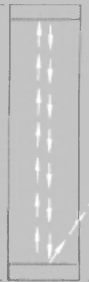
\includegraphics[scale=0.5]{LightClock}
\end{center}

A tick of the clock is given by the light travelling from the emitter,
bouncing off the upper mirror, and returning to the emitter/detector.
In $\S'$, the time for a single tick is given by
\[ \Delta t' = \frac{2\ell_0}{c} \]
In $\S$, though, it's a little more complicated. According to the stationary
referene frame, the light will be going travelling like so:
\begin{center}
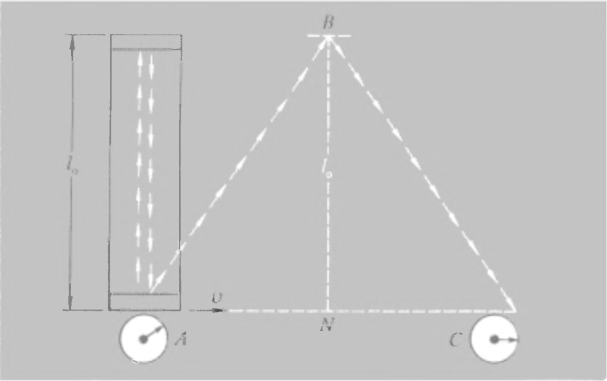
\includegraphics[scale=0.5]{Light}
\end{center}

In this case, we know the vertical length will always be $\ell_0$, and we can
say that each leg of the horizontal length should be $\frac{v\Delta t}{2}$.
The distance of each hypotenusal part of the light's journey should then be
$\sqrt{\ell_0^2 + (v\Delta t)^2}$. This means that the total time it takes
to travel both hypotenusal distances should be:
\begin{align*}
	\Delta t &=\frac{2\sqrt{\ell_0^2+\left(\frac{v\Delta t}{2}\right)^2}}
		{c}\\
	&= \frac{2}{c}\sqrt{\left(\frac{c\Delta t'}{2}\right)^2+\left(\frac{v
		\Delta t}{2}\right)^2}\\
	&= \frac{\Delta t'}{\sqrt{1 - \frac{v^2}{c^2}}}
\end{align*}
As we expect, these two times are different, which we would expect, given
our previous thought experiment. These two times leaves us with some
potentially confusing terminology when it comes to describing the time it takes
for something to happen. We refer to $\Delta t'$, the time it takes for
something to happen in the frame where it's stationary, as ``proper time'' to
make up for that.

\subsubsection{Definitions of Recurring Expressions}
\begin{align*}
	\beta &= \frac{v}{c}\\
	\gamma&=\frac{1}{\sqrt{1}-\frac{v^2}{c^2}} = \frac{1}{\sqrt{1-\beta^2}}
	&\text{``dilation factor''}
\end{align*}
Note that with this definition of $\gamma$, we can re-write time dilation as
$\Delta t = \gamma \Delta t'$, which is much simpler.

\subsubsection{Length Expansion and Contraction}
We can set up a similar situation, but this time, where the direction of the
light pulse in the light clock is parallel to the motion of the moving
frame $\S'$. Again, the clock is stationary in $S'$, where it has length
$\ell_0$. We can see easily that in $\S'$, the time for a single pulse
should be
\[ \Delta t' = \frac{2\ell_0}{c} \]
But since $c$ is the same in every frame, but the clock is moving in $\S$, to
find $\Delta t$, we must actually find two time differences in $\S$: one on
the way out, and one on the way in:
\begin{align*}
	\ell + v\Delta t_{out} = c&\Delta t_{out}\\
	\implies &\Delta t_{out}=\frac{\ell}{c-v}\\
	\ell - v\Delta t_{in} = c&\Delta t_{in}\\
	\implies &\Delta t_{in}=\frac{\ell}{c+v}
\end{align*}
Thus,
\begin{align*}
	\Delta t &= \Delta t_{out}+\Delta t_{in}\\
		 &= \frac{2\ell c}{c^2-v^2}\\
		 &= \frac{2\ell}{c}\gamma^2
\end{align*}
Since we know from before that $\Delta t = \gamma\Delta t'$, and that
$\Delta t' = \frac{2\ell_0}{c}$, we can conclude that
\begin{align*}
	\Delta t = \gamma \frac{2\ell_0}{c} &= \gamma^2\frac{2\ell}{c}\\
	\ell_0 &= \gamma\ell\\
	\ell &= \frac{\ell_0}{\gamma}
\end{align*}
The length of the clock in $\S$ is actually smaller than the length of the
clock in $\S'$. This is called length contraction, or Lorentz contraction.

\subsection{The Lorentz Transformations and Relattivistic Kinematics}
\subsubsection{Lorentz Transformations}
\begin{defi}[Event]
	An \emph{event} is any point in space and time which uniquely specifies
	all coordinates
\end{defi}

We will once again re-affirm our regular set-up. $\S$ is a stationary
inertial frame, and $\S'$ is an inertial from moving with a constant
velocity $v$ in the $x$ direction. Because there is no movement along the
$y$ or $z$ directions according to $\S$, we'll look only at the $x$
(and associated $x'$ directions for now. We can write a relationship between
the relative $x$ coordinates between the two frames in a way that mirrors the
Galilean transformation equations, and satisfies the requirement that they
must both still be in uniform rectilinear motion in both frames:
\begin{align*}
	x &= ax' + bt'\\
	x' &= ax - bt
\end{align*}
Our goal then is to find the unkonwn constants $a$ and $b$. We can find the
motion of the origin of $\S'$ relative to $\S$ by taking $x'=0$, and
visa-versa:
\begin{align*}
	0 = ax' + bt' &\implies x' = \frac{b}{a}t'\\
	0 = ax-bt &\implies x = \frac{b}{a}t
\end{align*}
These velocities are equal and opposite, of magnitude $v$. This tells us that
\[ \frac{b}{a} = v \]

Next, we can look at what happens to a light pulse moving in the positive
$x$ direction in each of these frames. We can describe this fairly
easily:
\begin{align*}
	x &= ct &&
	x' = ct'
\end{align*}
Substituting these into our equations from earlier, we find:
\begin{align*}
	ct = (ac+b)t' &&
	ct' = (ac-b)t
\end{align*}
We can eliminate and use our previous results to find that
\begin{align*}
	c^2 &= a^2(c^2-v^2)\\
	a &= \frac{1}{\sqrt{1-v^2/c^2}} = \gamma
\end{align*}
Thus, we can write the transformations for all 4 dimensions from $\S$ to
$\S'$, and from $\S'$ to $\S$, also called the \emph{Lorentz transformations}:
\begin{align*}
	x' &= \gamma(x-vt) & x &= \gamma(x'+vt')\\
	y' &= y & y &= y'\\
	z' &= z & z &= z'\\
	t' &= \gamma(t-vx/c^2) & t &= \gamma(t'+vx'/c^2)
\end{align*}

\subsubsection{Velocity Transformations}
We will now briefly discuss velocities relative to two inertial frames, namely
the velocities in the $x$ and $y$ directions. By definition of velocity, we can
define the $x$ and $y$ components of velocity in the $\S$ and $\S'$ frames
respectively as
\begin{align*}
	u_x = \der{x}{t} && u_y = \der{y}{t}\\
	u_x' = \der{x'}{t'} && u_y' = \der{y'}{t'}
\end{align*}
From differentiation of the Lorentz transformation equations, we can find that
\begin{align*}
	\d x &= \gamma(u_x')+v\d t'\\
	\d y &= u_y'\d t'\\
	\d t &= \gamma(1 + vu_x'/c^2)\d t'
\end{align*}
And so on. Thus,
\begin{align*}
	u_x &= \frac{u_x' + v}{1+vu_x'/c^2} &
		u_x' &= \frac{u_x-v}{1-vu_x/c^2}\\
	u_y &= \frac{u_y'/\gamma}{1+vu_x'/c^2} &
		u_y' &= \frac{u_y/\gamma}{1-vu_x/c^2}
\end{align*}
Note that because the Lorentz transformations for time depend on the relative
velocities in both inertial frames, velocity components in the $y$
(and, by extension, $z$) directions are changed as well. In the case of
$v\ll c$, these once again simplify to velocity transformations in Galilean
relativity.

\subsubsection{The Doppler Effect}


\subsubsection{Minkowski Diagrams}
Minkowski diagrams are graphs which allow us to easily represent a problem
in special relativity. In general, the horizontal axis is $x$ (or, more
generally, the relative dimension), and the vertical axis is $ct$. Note that
we use $ct$ rather than just $t$ here.
The path of a particle in spacetime is called its \emph{world line}.
We can draw the path of a single photon of light as a line with a $45^\circ$
angle between each set of axes. We define this as the world line of a photon.
The set of photon world lines is called the \emph{light cone}, and represents
the region of all possible paths of a particle starting at the origin, moving
at $v\leq c$. One
such diagram with a light cone is shown below.

\begin{center}                                                                
    \begin{tikzpicture}[scale=0.8]
      \draw [->] (-3, 0) -- (3, 0) node [right] {$x$};
      \draw [->] (0, -3) -- (0, 3) node [above] {$ct$};
      \draw [cyan] (-2.5, -2.5) -- (2.5, 2.5);
      \draw [cyan] (2.5, -2.5) -- (-2.5, 2.5);
    \end{tikzpicture}                                                           
\end{center}   

We can also use this to represent the relationship between two frames.
If we take this existing set of orthogonal axes to be the stationary frame
$\S$, then we can show the moving frame $\S'$ using a set of non-orthogonal
axes, using the Lorentz transformations to derive the slopes of these new
axis lines. In general, we can write
\begin{align*}
	x'=\gamma(x-\beta ct) && ct' = \gamma(ct-\beta x)
\end{align*}
There are two possibilities for a moving $\S'$:
\begin{enumerate}
	\item $\beta > 0$: The axes form an acute angle
	\item $\beta < 0$: The axes form an obtuse angle
\end{enumerate}
Note that the world line from the $\S$ frame still applies in the $\S'$ frame!
An example of a Minkowski diagram with two sets of axes is shown below.
\begin{center}                                                                  
  \begin{tikzpicture}[scale=0.8]                                                
    \draw [->] (-3, 0) -- (3, 0) node [right] {$x$};                      
    \draw [->] (0, -3) -- (0, 3) node [above] {$ct$};                     
    \draw [->, red] (-2.85, -0.8) -- (2.85, 0.8) node [right] {$x'$};           
    \draw [->, red] (-0.8, -2.85) -- (0.8, 2.85) node [above] {$ct'$};          
  \end{tikzpicture}                                                             
\end{center}

\begin{prop}
	The Lorentz invariant,
	\(S^2 = (ct)^2-x^2-y^2-z^2\), is invariant in all inertial frames.
\end{prop}
\begin{proof}
	If we start with two Lorentz invariants, one in $\S$ and one in
	$\S'$,
	\begin{align*}
		r^2 = x^2+y^2+z^2=(ct)^2 &&
	r'^2 = x'^2+y'^2+z'^2=(ct')^2
	\end{align*}
	and we insist that they be equal, then
\begin{align*}
	(ct')^2-x'^2-y'^2-z'^2 &= (ct)^2-x^2-y^2-z^2\\
	(ct')^2-x'^2-y'^2-z'^2 &= [\gamma(ct'-\beta x')]^2
		-[\gamma(x'-\beta ct')]^2-y^2-z^2\\
	(ct')^2-x'^2-y'^2-z'^2 &= \gamma^2[(ct')^2(1-\beta^2)+
		2(ct')x'\beta(-1+1)-x'^2(1-\beta^2)] -y^2-z^2\\
	(ct')^2-x'^2-y'^2-z'^2&=(ct')^2-x'^2-y'^2-z'^2
\end{align*}
\end{proof}

If we try to calculate the Lorentz invariant for a change in the $x$ and $ct$ 
directions, then we would get the equation for a hyperbola:
\[ S^2 = x'^2 - (ct')^2 = 1 \]
This is called the ``calibration hyperbola'' because it can show us (ie.
help us calibrate) the scale of a set of axes. Namely, a distance of 1 on some
distance axis (eg. $x$, $x'$, etc.) is given by the distance between the
origin and the point where the axis crosses the calibration hyperbola.
Below is a fuller Minkowski diagram. Note the shading: assuming something
starts at the origin, for it to occur in the undefined (gray)
regions, it would need to travelling faster than light in that direction, so
motion from the origin is bound within the world-lines in each direction.
This is true regardless of the reference frame we're in.

\begin{center}                                                                  
  \begin{tikzpicture}[scale=0.8]
  \fill[gray!15] (-3, 3) -- (0,0) -- (-3, -3) -- cycle;
  \fill[gray!15] (3, 3) -- (0,0) -- (3, -3) -- cycle;
    \draw [->] (-3, 0) -- (3, 0) node [right] {$x$};
    \draw [->] (0, -3) -- (0, 3) node [above] {$ct$};
    \draw [->, red] (-2.85, -0.8) -- (2.85, 0.8) node [right] {$x'$};
    \draw [->, red] (-0.8, -2.85) -- (0.8, 2.85) node [above] {$ct'$};
    \draw [cyan, dashed] (-3, -3) -- (3, 3);
    \draw [cyan, dashed] (3,-3) -- (-3, 3);
  \end{tikzpicture}                                                             
\end{center}

For two events, there are three possibilites, depending on the Lorentz
invariant:
\begin{enumerate}
	\item $S^2 > 0$: Time-like separated from the origin. The second
		event occurs at a different time than the origin and lies
		within the light cone
	\item $S^2 = 0$: Light-like separated from the origin. The second
		event lies on the light cone.
	\item $S^2 < 0$: Space-like separated from the origin. The second
		event occurs at a different point in space than the origin
		and lies outside the light cone.
\end{enumerate}

\subsection{Relativistic Dynamics}
\subsubsection{Energy, Momentum, and Mass}
I won't show the derivation exactly here, but one of Einstein's big discoveries
was that we could define the energy and mass of photons respectively as
\begin{align*}
	E = cp && m = \frac{E}{c^2}
\end{align*}
Combining these, we have
\[ m = \frac{p}{c} \]
This looks remarkably similar to how we could define mass in Newtonian
mechanics, as $m = \frac{p}{u}$. If we assume that this is, in fact, just
a particular case of standard Newtonian mass, and we assume that the energy
equation for a photon is universally true, we can find that
\[ E = \frac{c^2p}{u} \]
Classically, the increment of kinetic energy a particle gains or loses
due to some force is given by
\[ \d E = F\d x = \der{p}{t}\d x = u\d p \]
Combining this with our now-generalized expression for energy and integrating,
this means that
\begin{align*}
	E\d E &= c^2p\d p\\
	E^2 &= c^2p^2 + E_0^2
\end{align*}
Where $E_0^2$ is a constant of integration (which we've assumed to be the
square of some constant energy). From here, we can make some really cool
observations. First, let's use the equation for energy again and substitute
$cp = Eu/c$, to find that
\[ E(u) = \frac{E_0}{\sqrt{1-u^2/c^2}} = \gamma E_0 \]
For very low velocities, $v \ll c$, we can approximate this result to be
\[ E(u) \approx E_0 + \frac{1}{2}\frac{E_0}{c^2}u^2 \]
This looks pretty similar to the standard classical description, but it doesn't
quite fit. To make it fit, we have to link $\frac{E_0}{c^2}$ with the inertial
mass $m_0$. If we do say that those are equal, we can find another
equation to represent the energy, and do some more
algebraic trickery to define another form of inertial mass which varies
with speed:
\begin{align*}
	E(u) &= \gamma m_0 c^2 = (cp)^2 + m_0c^2\\
	m(u) &= \frac{m_0}{\sqrt{1-u^2/c^2}} = \gamma m_0
\end{align*}
This is also super important! This gives us a way to define momentum in
Special Relativity that doesn't break! Momentum is defined as
\[ \vec{p} = m(u)\vec{v} \]

Just to be sure, here's a list of all the cool stuff we discovered here that's
going to be super useful for our discussions of dynamics:
\begin{align*}
	m &= \gamma m_0\\
	\vec{p} &= \gamma m_0 \vec{u}\\
	E &= \gamma m_0 c^2
\end{align*}

\subsubsection{Elastic Collisions}


\subsubsection{Inelastic Collisions}

\section{Quantum Mechanics in Three Dimensions}
\subsection{Spherical Schr\"odinger Equation}
\subsubsection{The General Three-Dimensional Schr\"odinger Equation}
The generalized Schro\"odinger equation tells us that
\[ i\hslash\pder{\Psi}{t}=H\Psi \]
Where we can find the Hamiltonian operator $H$ given by
\[ H=\frac12 mv^2+V=\frac{1}{2m}(p_x^2+p_y^2+p_z^2)+V \]
We can use the definition of the momentum operators in the position space to
say that
\[ p_x \to \frac{\hslash}{i}\pd{x} \]
With similar results for $y$ and $z$, or
\[ \vec{p} \to \frac{\hslash}{i}\del \]
Thus,
\[ i\hslash\pder{\Psi}{t}=-\frac{\hslash}{2m}\nabla^2\Psi+V\Psi \]
Or, looking at the time-independent version of this equation,
\[ -\frac{\hslash^2}{2m}\nabla^2\psi + V\psi = E\psi \]
Meaning we can write
\begin{align*}
	\Psi_n(\vec{r},t) &= \psi_n(\vec{r})e^{-iE_nt/\hslash}\\
	\Psi(\vec{r},t)&=\sum c_n\psi_n(\vec{r})e^{-iE_nt/\hslash}
\end{align*}
Where $c_n$ is determined by the initial/boundary conditions. The normalization
condition is given by
\[ \int\lvert\Psi\rvert^2\d^3\vec{r} = 1 \]
Where $\d^3\vec{r}$ depends on the coordinate system, but can be written in
Cartesian coordinates as $\d^3\vec{r}=\d x\d y\d z$

\subsubsection{The Three-Dimensional Schr\"odinger Equation in Spherical
Coordinates}
In spherical coordinates, the Laplacian takes the form
\[ \nabla^2 = \frac{1}{r^2}\pd{r}\left(r^2\pd{r}\right) +\frac{1}
{r^2\sin\theta}\pd{\theta}\left(\sin\theta\pd{\theta}\right)+
\frac{1}{r^2\sin^2\theta} \left(\pder{^2}{\phi^2}\right)\]
So in spherical coordinates, the time-independent Schr\"odinger equation can
be written as
\[ -\frac{\hslash^2}{2m}\left[
\frac{1}{r^2}\pd{r}\left(r^2\pder{\psi}{r}\right) +\frac{1}
{r^2\sin\theta}\pd{\theta}\left(\sin\theta\pder{\psi}{\theta}\right)+
\frac{1}{r^2\sin^2\theta} \left(\pder{\psi^2}{\phi^2}\right)\right] + V\psi
= E\psi
\]

We can use the method of separation of variables to solve this, using an
ansatz of
\[ \psi(r,\theta,\phi) = R(r)Y(\theta,\phi) \]

If we substitute this into the spherical Schr\"odinger equation, and simplify
by dividing by $RY$ and multiplying by $-2mr^2/\hslash^2$, then we would get
\[
	\left\{\frac{1}{R}\pd{r}\left(r^2\pder{R}{r}\right)-
	\frac{2mr^2}{\hslash^2}[V(r)-E]\right\} +
	\frac{1}{Y}\left\{\frac{1}{\sin\theta}\left(\sin\theta\pder{Y}{\theta}
	\right)+\frac{1}{\sin^2\theta}\pder{^2Y}{\phi^2}\right\}
	=0
\]
We can see that the first bracketed term depends only on $r$, and the second
term depends only on $\theta$ and $\phi$, so each must be a constant. We'll
write the constant in the form $\ell(\ell+1)$.

\paragraph{The Angular Equation and Spherical Harmonics}
Simplified, the angular equation is given by
\[
	\frac{1}{Y}\left\{\frac{1}{\sin\theta}\left(\sin\theta\pder{Y}{\theta}
	\right)+\frac{1}{\sin^2\theta}\pder{^2Y}{\phi^2}\right\}=-\ell(\ell+1)
\]
As we've seen in Math Methods, this differential equation is best solved using
spherical harmonics. If we separate $Y$ again using the separation of variables
method to find another separation consntant, $m$, then we find that
\[ Y(\theta,\phi) = Y_\ell^m(\theta,\phi) \]

\paragraph{The Radial Equation}
Simplified, the radial equation is given by
\[
	\pd{r}\left(r^2\pder{R}{r}\right)-\frac{2mr^2}{\hslash^2}[V(r)-E]R
	= \ell(\ell+1)R
\]
If we use a change of variables, $u(r)\equiv rR(r)$, then we can simplify this
equation (using a whole lot of chain rule) to
\begin{align*}
	-\frac{\hslash^2}{2m}\der{^2u}{r^2}+\left[V+\frac{\hslash^2}{2m}
	\frac{\ell(\ell+1)}{r^2}\right]u=Eu
\end{align*}
We'll always assume that the potential we're given is a central potential.
This is called the radial equation, and it is basically identical to the
one-dimensional equation, except that the potential has an extra so-called
centrifugal term. Because of that, we can call this the effective
one-dimensional Schr\"odinger equation, and the new extra-term potential
the effective potential:
\[ V_{eff}=V+\frac{\hslash^2}{2m}\frac{\ell(\ell+1)}{r^2} \]
The normalization condition becomes
\[ \int_0^\infty \lvert u \rvert^2\d r=1 \]

\subsubsection{The Free Particle}
For a free particle, $V(r)=0$. We can use $R(r)$ rather than $u(r)$ for this
problem because the solutions will be simpler that way. We know that the
radial Schr\"odinger equation will look like
\[
	\pd{r}\left(r^2\pder{R}{r}\right)-\frac{2mr^2}{\hslash^2}ER
	= \ell(\ell+1)R
\]
We know that \[E=\frac{\hslash^2\kappa^2}{2m}\]
Since $\kappa$ has units of m$^{-1}$, we can define the dimensionless constant
$x=\kappa r$, and substitute these both in the effectuve 1D equation. If we
do this and simplify, we find that
\[
	x^2\pder{^2R}{x^2}+2x\pder{R}{x}+[x^2-\ell(\ell+1)]R=0
\]
This looks a lot like Bessel's equation! But it's not quite. If we do another
change of variables, $R(x) = x^{-1/2}y(x)$, then we can re-write this equation
as
\[ x^2y''(x)+xy'(x)+[x^2-(\ell+1/2)^2]y(x)=0\]
This means that we can write the two types of solutions as
\begin{align*}
	R(r) = 
	\begin{cases}
		\frac{1}{\sqrt{x}}J_{\ell+1/2}(x)\\
		\frac{1}{\sqrt{x}}N_{\ell+1/2}(x)
	\end{cases}
	=
	\begin{cases}
		\sqrt{\frac{2}{\pi}}j_{\ell}(x)\\
		\sqrt{\frac{2}{\pi}}n_{\ell}(x)
	\end{cases}
\end{align*}
Where $j_{\ell}(x)$ and $n_{\ell}(x)$ are the Spherical Bessel functions,
defined as
\begin{align*}
	j_{\ell}(x) = \sqrt{\frac{\pi}{2x}}J_{\ell+1/2}(x) &&
	n_{\ell}(x) = \sqrt{\frac{\pi}{2x}}N_{\ell+1/2}(x)
\end{align*}

The angular equation will still be spherical harmonics.

\subsubsection{The Infinite Spherical Well}
In an infinite spherical well,
\begin{align*}
	V(r) = 
\begin{cases}
	0, & r\leq a\\
	\infty, & r>a
\end{cases}
\end{align*}

Outside the well,
\[ \psi(r) = 0\]

Inside, the well, the radial equation comes out to
\[ \pder{^2u}{r^2}=\left[\frac{\ell(\ell+1)}{r^2}-k^2\right]u \]
where
\[ k\equiv\frac{\sqrt{2mE}}{\hslash} \]
Per the last section, we can do some algebraic magic to find that the general
solution to this is
\[ u(r) = Arj_{\ell}(kr)+Brn_{\ell}(kr) \]
At the origin, Bessel functions are finite, but Neumann functions blow up,
so we must take $B=0$ since we expect the wave function to be finite at the
origin. Thus, we can say that
\begin{align*}
	u(r) &= Arj_{\ell}(kr)\\
	\implies R(r)&=Aj_{\ell}(kr)
\end{align*}
We have to find reasonable values for $k$ still, but unfortunately, the zeroes
of spherical Bessel functions aren't predictable and have to instead be
calculated manually. The boundary condition $R(a)=0$ requires that
\[ k = \frac{1}{a}\beta_{n\ell} \]
Where $\beta_{n\ell}$ is the $n^{th}$ zero of the $\ell^{th}$ Bessel function.
We can extrapolate to say that the allowed energies are the given by
\[ E_{n\ell}=\frac{\hslash^2}{2ma^2}\beta^2_{n\ell} \]
The angular equation will still come out to spherical harmonics, so the full
wave functions can be given by
\begin{align*}
\psi_{n\ell m}(r,\theta,\phi) &= A_{n\ell}j_{\ell}(kr)Y_\ell^m(\theta,\phi)\\
			      &= A_{n\ell}j_{\ell}
		\left(\beta_{n\ell}\frac{r}{a}\right)Y_\ell^m(\theta,\phi)
\end{align*}
Where $A_{n\ell}$ can be determined with normalization. Each energy level will
be $(2\ell+1)$-fold degernate, since there are that many $m$ values for each
$\ell$ value.

\subsubsection{The Spherical Harmonic Oscillator}

\subsection{The Hydrogen Atom}
The hydrogen atom consists, essentially, of a motionless proton at the origin
with charge $e$, and a very light electron with charge $-e$ orbiting it.
We can write the potential and Schr\"odinger's equations for this:

\[
	V(r) = -\frac{e^2}{4\pi\epsilon_0}\frac{1}{r}
\]
\[
	-\frac{\hslash^2}{2m}\der{^2u}{r^2}+\left[-\frac{e^2}{4\pi\epsilon_0}
	\frac{1}{r}+\frac{\hslash^2}{2m}\frac{\ell(\ell+1)}{r^2}\right]u
	= Eu
\]

\subsubsection{The Solution}
Because we have a central potential (dependent only on $r$), we know from
the previous examples that the solution will look like
\begin{align*}
	\Psi_{n\ell m}(r,\theta,\phi)&=R_{n\ell}(r)Y_\ell^m(\theta,\phi)\\
				     &=\frac{u(r)}{r}Y_\ell^m(\theta,\phi)
\end{align*}
We, then, are tasked with finding $u(r)$.

\subsubsection{The Radial Wave Function}
First, let's make some variable changes to make htis look a little nicer.
We'll define a constant \[ \kappa \equiv \frac{\sqrt{-2mE}}{\hslash} \]
Then, we can define a variable and another constant that depends on $\kappa$:
\begin{align*}
	\rho &\equiv \kappa r\\
	\rho_0 &\equiv \frac{me^2}{2\pi\epsilon_0\hslash^2\kappa}
\end{align*}
This way, we can re-write the spherical Schr\"odinger equation such that
\[ \der{^2u}{\rho^2}=
\left[1-\frac{\rho_0}{\rho}+\frac{\ell(\ell+1)}{\rho^2}\right] u \]

We know our boundary conditions,
\begin{enumerate}
	\item $u(\rho\to\infty) = 0$
	\item $u(\rho\to0) = 0$
\end{enumerate}

Starting with (i), if we take $\rho\to\infty$, the $\frac{1}{\rho}$ and
$\frac{1}{\rho^2}$ terms will fall away, so the equation becomes approximately
\[ \der{^2u}{u^2} = u \]
Which we know and can write the general solution to:
\[ u(\rho) = Ae^{-\rho} + Be^{\rho} \]
But! To fit this boundary condition, we require that $u(\infty)=0$, so
we must have $B=0$, meaning for a large $\rho$,
\[u(\rho) \approx Ae^{-\rho}\]

Next, using (ii), when $\rho\to0$, the centrifugal term (that is, the
$\frac{1}{\rho^2}$ term) dominates, meaning the equation can be simplified to
\[ \der{^2u}{\rho^2} = \frac{\ell(\ell+1)}{\rho^2}u \]
The general solution for this differential equation is a bit more difficult to
find, but if we do the legwork, it comes out to
\[ u(\rho) = C\rho^{\ell+1}+D\rho^{-\ell} \]
But! Since we need this to equal 0 as $\rho\to0$, we can set $D=0$, and thus
for small $\rho$,
\[ u(\rho) \approx C\rho^{\ell+1} \]

So, we're left with the behavior of the function at each asymptote, but we
need a tapering function in the middle to help it smoothly transition to each
of these end-behavior functions. We can write this as $v(\rho)$ and let it
absorb the constants $A$ and $C$, such that
\[ u(\rho) = \rho^{\ell+1}e^{-\rho}v(\rho) \]
In terms of $v(\rho)$, the raidial equation we're left with is then
\[ \rho \der{^2v}{\rho^2}+2(\ell+1-\rho)\der{v}{\rho}+[\rho_0-2(\ell+1)]v=0 \]
We can use the method of Frobenius to guess a solution as a power series:
\[ v(\rho) = \sum_{j=0}^{\infty} c_j\rho^j \]
If we differentiate this twice and plug it into the radial equation in terms of
$v(\rho)$, we can find that
\[ c_{j+1} = \left[\frac{2(j+\ell+1)-\rho_0}{(j+1)(j+2\ell+2)}\right]c_j\]

The issue: this doesn't converge. We can prove that with some fancy estimating,
or you can just take my word for it. Since this doesn't converge, but we need
$u$ to converge to 0 at very small and very large $\rho$ values, there must be
some $j_{max}$ such that $c_{j>j_{max}}=0$.

By the recursive definition of $c_j$, this means that
\[ 2(j_{max}+\ell+1)-\rho_0 = 0 \]
We can (and will) define the \emph{principle quantum number} $n$ as
$n \equiv j_{max}+\ell+1$, so that
\[ \rho_0 = 2n \]
Since we already have an equation for $\rho_0$, which determines $E$, we can
use this to solve for the allowed values of $E$:
\[ E_n = -\left[\frac{m}{2\hslash^2}\left(\frac{e^2}{4\pi\epsilon_0}\right)^2
\right]\frac{1}{n^2} = \frac{E_1}{n^2} \]
This is also called \emph{Bohr's formula}.
We can also combine these formulas
to find
\[ \kappa = \left(\frac{me^2}{4\pi\epsilon_0\hslash^2}\right)\frac{1}{n}=
\frac{1}{an} \]
where
\[a \equiv \frac{4\pi\epsilon_0\hslash}{me^2} = 0.529\times10^{-10}\mathrm{m}\]
is called the \emph{Bohr radius}, and is the most likely value for the distance
from the proton to the electron.

It follows that
\[ \rho = \frac{r}{an} \]
Thus, the wave functions for the hydrogen atoms are marked by 3 quantum
numbers, $n$, $\ell$, and $m$, and can be written (as we saw before) as
\[ \psi_{n\ell m}(r,\theta,\psi) = R_{n\ell}(r)Y_\ell^m(\theta,\psi) \]
Where
\[ R_{n\ell}(r) = \frac{1}{r}\rho^{\ell+1}e^{-\rho}v(\rho)\]
Where $v(\rho)$ is a polynomial of degree $j_{max}=n-\ell-1$, whose
coefficients are given by the recursion formula from earlier.

If we assume that $j_{max} \geq 0$, then we can say that
\[ n \geq \ell + 1 \implies \ell \leq n - 1 \]

\subsubsection{The Ground State of the Hydrogen Atom}
The ground state of the hydrogen atom is the lowest physically-allowed energy
state, or $n=1$. At $n=1$,
\[ E_1 = -\left[\frac{m}{2\hslash^2}\left(\frac{e^2}{4\pi\epsilon_0}\right)
\right] = -13.6 \mathrm{eV} \]
The ground state has no degernacies. Based on what we know about the
relationship between $n$ and $\ell$, and the relationship between $\ell$ and
$m$, the only allowed values for $\ell$ and $m$ are $\ell=m=0$. Thus, the
ground-state wave function for a Hydrogen atom is given by
\begin{align*}
	\psi_{100}(r,\theta,\phi) &= R_{10}Y_0^0(\theta,\phi)\\
				  &= \frac{1}{\sqrt{\pi a^3}}e^{-r/a}
\end{align*}

\subsubsection{Laguerre Equations}
The second-order differential equation that we found earlier in terms of
$v(\rho)$,
\[ \rho\der{^2v}{\rho^2} = +2(\ell+1-\rho)\der{v}{\rho}+2(n-\ell-1)=0 \]
is also called the ``Associated Laguerre equations,'' whose solutions are the
Associated Laguerre Polynomials, gien by
\begin{align*}
	L_{q-p}^p(x) &= (-1)^p\left(\frac{\d}{\d x}\right)^p L_q(x)\\
	L_{q}(x) &= e^x\left(\frac{\d}{\d x}\right)^q(e^{-x}x^q)
\end{align*}
Substituting this in, the normalized wave function for the hydrogen atom is
given by
\[ \psi_{n\ell m} =
	\sqrt{\left(\frac{2}{na}\right)^3\frac{(n-\ell-1)!}{2n[(n+\ell)!]^3}}
	e^{-r/na}\left(\frac{2r}{na}\right)^\ell
		\left[L_{n-\ell-1}^{2\ell+1}(2r/na)\right] Y_\ell^m(\theta,\phi)
\]

\subsubsection{The Energy Spectrum of Hydrogen}
[Come back to this]

\subsection{Angular Momentum}
In classical mechanics, we have a definition of angular momentum given by
\begin{align*}
	\vec{L} &= \vec{r}\times\vec{p}\\
	L_x &= yp_z-zp_y\\
	L_y&=zp_x-xp_z\\
	L_x&=xp_y-yp_x
\end{align*}
We can turn these into quantum operators by using the standard prescription for
momentum and position.
\begin{align*}
p_{x_n} &\to -i\hslash\pd{x_n}\\
\implies \vec{p} &\to -i\hslash\del\\
x_n &\to x_n
\end{align*}
We can use this to re-write
\begin{align*}
	L &\to i\hslash\vec{r}\times\del\\
	L_i &\to -i\hslash\epsilon_{ijk}x_j\pd{k}\\
	    &\to \epsilon_{ijk}x_jp_k\\
	L_z &\to -i\hslash\left(x\pd{y}-y\pd{x}\right)
\end{align*}

\subsubsection{Angular Momentum Eigenvalues}
We can find easily (I'm not going to do all the math right now) that the
angular momentum operators fail to commute with the operators for any direction
other than their own:
\begin{align*}
	[L_x,L_y] &= i\hslash L_z\\
	[L_y,L_z] &= i\hslash L_x\\
	[L_z,L_x] &= i\hslash L_y
\end{align*}
This means that $L_x$, $L_y$, and $L_z$ are incompatible observables. According
to the generalized uncertainty principle,
\[ \Delta L_x \Delta L_y \geq \frac{\hslash}{2}\lvert\langle L_z\rangle\rvert\]
This shows us that it would be useless to look for states that are eigenstates
of $L_x$ and $L_y$ simultaneously.o

We can show that $L^2 \equiv L_x^2+L_y^2+L_z^2$ \emph{does} commute with
any individual angular momentum operator, though:
\begin{align*}
	[L^2,L_x] &= 0\\
	[L^2,L_y] &= 0\\
	[L^2,L_z] &= 0\\
	[L^2, \vec{L}] &= 0
\end{align*}
Since $L^2$ does commute with any of these, we can hope to find simultaneous
eigenstates of $L^2$ and, say, $L_z$, such that
\begin{align*}
	L^2\bket{\lambda,\mu} &= \lambda\bket{\lambda,\mu}\\
	L_z\bket{\lambda,\mu} &= \mu\bket{\lambda,\mu}
\end{align*}

To find the eigenalues and eigenfunctions, we'll use the ladder operator
technique, like how we did in PHY314 with the harmonic oscillator.
We can define
\[ L_{\pm} = L_x \pm iL_y \]
If we do, we can find that
\begin{align*}
	[L_z,L_{\pm}] &= \pm\hslash L_{\pm}\\
	[L^2,L_{\pm}] &= 0\\
	L_\pm L_\mp &= L^2-L_z^2\mp i(i\hslash L_z)\\
	\implies L^2 &= L_\pm L_\mp + L_z^2 \mp \hslash L_z
\end{align*}

Claim: If $\bket{\lambda,\mu}$ is an eigenfunction of $L^2$ and $L_z$, so is
$L_{\pm}\bket{\lambda,\mu}$. We can prove this easily for both cases:
\begin{align*}
L^2(L_\pm\bket{\lambda,\mu}) &= L_\pm(L^2\bket{\lambda,\mu})\\
			     &= L_\pm (\lambda\bket{\lambda,\mu})\\
			     &= \lambda(L_\pm\bket{\lambda,\mu})\\~\\
L_z(L_{\pm}\bket{\lambda,\mu})&=([L_z,L_\pm]+L_\pm L_z)\bket{\lambda,\mu}\\
			      &=(\pm\hslash L_\pm+\mu L_\pm)\bket{\lambda,\mu}\\
			      &= (\mu\pm\hslash)(L_\pm\bket{\lambda,\mu})
\end{align*}
So $L_\pm\bket{\lambda,\mu}$ is an eigenstate of $L^2$ with the same
eigenvalue $\lambda$, and is an eigenstate of $L_z$ with a slightly increased
or decreased eigenvalue of $\mu \pm \hslash$. Thus, for any given $\lambda$,
we can obtain a ``ladder'' of $\mu$ states, separated by $\hslash$,
obtained by applying the ladder operators to $\bket{\lambda,\mu}$. Obviously,
though, there must be some limit on this. We cannot have the z-component of
angular momentum exceed the total angular momentum, meaning there must be
some maximum such that
\[ L_+\bket{\lambda,\mu_{max}} = 0 \]
We'll define \[\mu_{max} = \hslash\ell\] meaning we can write this state as
\begin{align*}
	L_z\bket{\lambda,\hslash\ell}&=\hslash\ell\bket{\lambda,\hslash\ell}\\
	L^2\bket{\lambda,\hslash\ell}&=\lambda\bket{\lambda,\hslash\ell}
\end{align*}
By the relation of $L^2$ and $L_\pm L\mp$ that we claimed earlier, we can say
that
\begin{align*}
	L^2\bket{\lambda,\hslash\ell}&=
		(L_-L_+ + L_z^2+\hslash L_z)\bket{\lambda,\hslash\ell}\\
		&=(0+\hslash^2\ell^2+\hslash^2\ell)\bket{\lambda,\hslash\ell}\\
		&= \hslash^2\ell(\ell+1)
\end{align*}
Which tells us that $\lambda=\hslash^2\ell(\ell+1)$, or the eigenvalue of
$L^2$ in terms of the maximum eigenvalue of $L_z$. We can apply the same
process to the bottom-most state:
\begin{align*}
	L_-\bket{\lambda,\hslash\bar{\ell}}&=0\\
	L_z\bket{\lambda,\hslash\bar{\ell}}&=
		\hslash\bar{\ell}\bket{\lambda,\hslash\bar{\ell}}\\
	L^2\bket{\lambda,\hslash\bar{\ell}}&=
		\lambda\bket{\lambda,\hslash\bar{\ell}}\\~\\
	L^2\bket{\lambda,\hslash\bar{\ell}} &=
		(L_+ L_- + L_z^2-\hslash L_z)\bket{\lambda,\hslash\bar{\ell}}\\
		&=(0+\hslash^2\bar{\ell}^2-\hslash^2\bar{\ell})
			\bket{\lambda,\hslash\bar{\ell}}\\
	&= \hslash^2\bar{\ell}(\bar{\ell}-1)\bket{\lambda,\hslash\bar{\ell}}\\
	\implies \lambda &= \hslash^2\bar{\ell}(\bar{\ell}-1)
\end{align*}
Both of these things are simultaneously true, meaning we can find a
relationship between $\ell$ and $\bar{\ell}$:
\[ \bar{\ell} = -\ell \]
So, the eigenvalues of $L_z$ should be $m\hslash$, where $m$ can vary from
$-\ell\to\ell$ in $N$ integer steps. It follows that 
\[ \ell=-\ell+N \implies \ell=N/2 \]
and so $\ell$ must be either an integer or a half-integer. We can characterize
the eigenfunctions instead, then, as
\begin{align*}
	L^2\bket{m,\ell} &= \hslash^2\ell(\ell+1)\bket{m,\ell}\\
	L_z\bket{m,\ell} &= \hslash m\bket{m,\ell}
\end{align*}
Note that for a given $\ell$ value, there are $2\ell+1$ possible states.

\subsubsection{Angular Momentum Eigenfunctions}
We want to write
\[ \braket{\vec{r}}{\ell,m} \]
or the eigenfunctions of angular momenta in position space. First, we want
to write the angular momentum operators themselves in terms of spherical
coordinates:
\begin{align*}
	\vec{L} &= -i\hslash\vec{r}\times\del\\
	\del &= \hat{r}\pd{r}+\hat{\theta}\frac{1}{r}\pd{\theta}+\hat{\phi}
	\frac{1}{r\sin\theta}\pd{\phi}
\end{align*}
\begin{align*}
	\vec{L} &= -i\hslash\left[r(\hat{r}\times\hat{r})\pd{r} +
		(\hat{r}\times\hat{\theta})\pd{\theta}+
		(\hat{r}\times\hat{\phi})\frac{1}{\sin\theta}\pd{\phi}
	\right]\\
	&= -i\hslash\left(\phi\pd{\theta}-\hat{\theta}\frac{1}{\sin\theta}
	\pd{\theta}\right)\\
	&= -i\hslash\left[(-\sin\phi\hat{x}+\cos\phi\hat{y})\pd{\theta}-
	(\cos\theta\cos\phi\hat{x}+\cos\theta\sin\phi\hat{y}-\sin\theta\hat{z})
	\frac{1}{\sin\theta}\pd{\phi}\right]
\end{align*}
\begin{align*}
	L_x &= -i\hslash\left(-\sin\phi\pd{\theta}-\cos\phi\cot\theta\pd{\phi}
	\right)\\
	L_y &= -i\hslash\left(\ \ \ \cos\phi\pd{\theta}-\sin\phi\cot\theta
	\pd{\phi}\right)\\
	L_z &= -i\hslash\pd{\phi}
\end{align*}
We can also find the position-space representation of the ladder operators
using the identity $\cos\phi\pm i\sin\phi = e^{\pm i\phi}$ (I won't show the
full work here), and from there, find a representation of $L^2$:
\begin{align*}
	L_\pm &= \pm\hslash e^{\pm i\phi}\left( 
		\pd{\theta}\pm i\cot\theta\pd{\phi}
	\right)\\
	L^2 &= -\hslash^2\left[\frac{1}{\sin\theta}\pd{\theta}\left(
	\sin\theta\pd{\theta}\right)+\frac{1}{\sin^2\theta}\pder{^2}{\phi^2}
	\right]
\end{align*}
Okay. Now we're finally ready to find the eigenfunctions of $L^2$ with
eigenvalues $\hslash^2\ell(\ell+1)$. But note--this equation we've just found
for $L^2$ is just the equation for spherical harmonics! So that means that
\[ \braket{\vec{r}}{m,\ell} = Y_m^\ell(\theta,\phi) \]
Important note: using this solution, $\ell$ (and therefore $m$) can only take
integer values---half-integer values would imply that
$Y_\ell^m(\theta,0) \neq Y_\ell^m(\theta,2\pi)$, which can't be true.

\subsection{Spin}
In classical mechanics we make a fairly meaningless distinction between
orbital angular momentum, the angular momentum of the center of mass, and spin
angular momentum, the momentum about the center of mass. In quantum mechanics,
we make a similarly-labelled and very meaningful distinction, although what
we'll call ``spin'' is actually just an intrinsic angular momentum-like thing,
not something that's actually reliant on some type of motion of the particles.

\subsubsection{Foundations}

The foundations for the spin operators, $\vec{S}$, are pretty much exactly the
same as with $\vec{L}$:
\begin{align*}
	[S_i,S_j]&=i\hslash\epsilon_{ijk}S_k\\
	S^2\bket{s,m} &= \hslash^2 s(s+1)\bket{s,m}\\
	S_z\bket{s,m} &= \hslash m\bket{s,m}\\
	S_\pm\bket{s,m}&=\hslash\sqrt{s(s+1)-m(m\pm1)}\bket{s,m\pm1}
\end{align*}
The big difference with spin, is that the eigenfunctions are not spherical
harmonics, so there's no immediate reason to exclude half-integer values
of $s$ and $m$. It turns out, every type of elementary particle has a specific
and unchangeable $s$ value, which we call the spin of that type of particle.

\subsubsection{Spin 1/2}
The most important case is $s=1/2$, since this is the spin of most important
elementary particles we deal with (protons, neutrons, electrons) and also
quarks and leptons. There are 2 potential eigenstates for $s=1/2$:
\begin{align*}
	&\bket{\frac12,\frac12} &\implies &\text{``Spin Up,'' }\uparrow\\
	&\bket{\frac12,-\frac12} &\implies &\text{``Spin Down,'' }\downarrow
\end{align*}
Using this basis, we can represent the general state of a spin-1/2 particle
as a two-element vector called a \emph{spinor}:
\begin{align*}
	\chi &= \begin{pmatrix}a\\b\end{pmatrix}
	     = a\chi_++b\chi_-\\
	\chi_+ &= \begin{pmatrix}1\\0\end{pmatrix}\\
	\chi_- &= \begin{pmatrix}0\\1\end{pmatrix}
\end{align*}
Where $\chi_+$ represents ``spin up'' and $\chi_-$ represents ``spin down.''

Using this notation, the operators become 2$\times$2 matrices, which we can
find! By the definition of the $S^2$ operator, we know that
\begin{align*}
	\matr{S}^2\chi_+ &= \frac34\hslash^2\chi_+\\
	\matr{S}^2\chi_- &= \frac34\hslash^2\chi_-
\end{align*}
If we write $\matr{S}^2$ as a matrix with undetermined coefficients, this is
a pretty easily-solved system:
\[ \matr{S}^2 = \begin{pmatrix}c&d\\e&f\end{pmatrix} \]
\begin{align*}
	\begin{pmatrix}c&d\\e&f\end{pmatrix}
	\begin{pmatrix}1\\0\end{pmatrix}
	&=\frac34\hslash^2\begin{pmatrix}1\\0\end{pmatrix}\\
	\implies \begin{pmatrix}c\\e\end{pmatrix}&=
	\begin{pmatrix}\frac34\hslash^2\\0\end{pmatrix}\\~\\
	\begin{pmatrix}c&d\\e&f\end{pmatrix}
	\begin{pmatrix}0\\1\end{pmatrix}
	&=\frac34\hslash^2\begin{pmatrix}0\\1\end{pmatrix}\\
	\implies \begin{pmatrix}d\\f\end{pmatrix}&=
	\begin{pmatrix}0\\\frac34\hslash^2\end{pmatrix}\\
\end{align*}
\[ \matr{S}^2 = \frac34\hslash^2\begin{pmatrix}1&0\\0&1\end{pmatrix} \]
We can use a similar to process to show that
\[ \matr{S}_z = \frac{\hslash}{2}\begin{pmatrix}1&0\\0&-1\end{pmatrix} \]
We can use a similar process again to find the matrix representation of the
ladder operators, and by extension, the $x$ and $y$ spin operators:
\begin{align*}
	\matr{S}_+ &= \hslash\begin{pmatrix}0&1\\0&0\end{pmatrix}\\
	\matr{S}_- &= \hslash\begin{pmatrix}0&0\\1&0\end{pmatrix}\\
	\matr{S}_x &= \frac{\hslash}{2}\begin{pmatrix}0&1\\1&0\end{pmatrix}\\
	\matr{S}_y &= \frac{\hslash}{2}\begin{pmatrix}0&-i\\i&0\end{pmatrix}\\
\end{align*}
Since $\matr{S}_x$, $\matr{S}_y$, and $\matr{S}_z$ all have a factor of
$\hslash/2$, it can be easier to write
$\vec{S} = \frac{\hslash}{2}\vec{\sigma}$, where $\vec{sigma}$ are the Pauli
spin matrices:
\begin{align*}
	\sigma_x &= \begin{pmatrix}0&1\\1&0\end{pmatrix}\\
	\sigma_y &= \begin{pmatrix}0&-i\\i&0\end{pmatrix}\\
	\sigma_z &= \begin{pmatrix}1&0\\0&-1\end{pmatrix}\\
\end{align*}

The eigenspinors of $\matr{S}_z$ for the eigenvalues $\frac{\hslash}{2}$ and
$-\frac{\hslash}{2}$, respectively, are given by $\chi_+$ and $\chi_-$. When
youe measure the z-component of a particle's spin, you could get
eigenvalue $\hslash/2$ with probability $\abs{a}^2$ or eigenvalue
$-\hslash/2$ with probability $\abs{b}^2$. Since these are the only
possibilities, \[ \abs{a}^2+\abs{b}^2=1 \] Meaning the spinor
$\chi = a\chi_++b\chi_-$ must be normalized.

But what if we want to meaasure $S_x$ instead? The characteristic equation to
determine the eigenvalues is given by
\begin{align*}
	\begin{vmatrix}-\lambda&\hslash/2\\\hslash/2&-\lambda\end{vmatrix}&=0\\
	\lambda^2&=\left(\frac{\hslash}{2}\right)^2\\
	\lambda&=\pm\frac{\hslash}{2}
\end{align*}
The eigenspinors can be obtained by solving the eigenvalue equation to find
\begin{align*}
	\chi_+^{(x)}
	&=\begin{pmatrix}\frac{1}{\sqrt{2}}\\\frac{1}{\sqrt{2}}\end{pmatrix}\\
	\chi_-^{(x)}
	&=\begin{pmatrix}\frac{1}{\sqrt{2}}\\-\frac{1}{\sqrt{2}}\end{pmatrix}
\end{align*}
These span the entire space, meaning the generic spinor can be written as a
linear combination of them. Specifically,
\[ \chi = \left(\frac{a+b}{\sqrt{2}}\right)\chi_+^{(x)} +
\left(\frac{a-b}{\sqrt{2}}\right)\chi_-^{(x)} \]

\subsubsection{Electrons in a Magnetic Field}
A charged particle that's spinning makes a magnetic dipole, whose dipole
moment is proportional to its spin angular momentum:
\[ \vec{\mu} = \gamma\vec{S} \]
Where $\gamma$ is called the gyromagnetic ratio.

When this dipole is placed in a magnetic fiwld, it experiences a torque
aligning it (generally) parallel to the field, given by
\[ \vec{\tau} = \vec{\mu}\times\vec{B} \]
The energy associated with $\vec{\tau}$ is
\[ H = -\vec{\mu}\cdot\vec{B} \]
So the Hamiltonian of a spinning charged particle at rest in a magnetic field
is given by
\[ H = -\gamma\vec{B}\cdot\vec{S} \]

\subsubsection{Addition of Angular Momenta}

Let's say we have a hydrogen atom whose electron and proton are in the ground
state. This means we have two 1/2-spin particles with no orbital angular
momentum. What is the total angular momentum? Let
$\vec{S}=\vec{S}^{(1)}+\vec{S}^{(2)}$, where (1) refers to the proton, and
(2) refers to the electron.

There are four possible states (really, the system is a linear combination
of these states): $\uparrow\uparrow$, $\uparrow\downarrow$,
$\downarrow\uparrow$, and $\downarrow\downarrow$. Each of these states is an
eigenstate of $S_z$, and the $z$ components can be added by the principle of
superposition:
\begin{align*}
	S_z\chi_1\chi_2 &= (S_z^{(1)}+S_z^{(2)})\chi_1\chi_2\\
			&= (S_z^{(1)}\chi_1)\chi_2+\chi_1(S_z^{(2)}\chi_2)\\
			&= (\hslash m_1\chi_1)\chi_2+\chi_1(\hslash m_2\chi_2)\\
			&= \hslash(m_1+m_2)\chi_1\chi_2
\end{align*}
So the quantum number for the spin is simply $m=m_1+m_2$. The quantum number
for each state can be easily found then:
\begin{align*}
	\uparrow\uparrow: m&=1\\
	\uparrow\downarrow: m&=0\\
	\downarrow\uparrow: m&=0\\
	\downarrow\downarrow: m&=-1
\end{align*}

\section{Quantum Mechanics for Identical Particles}

\subsection{Two-Particle Systems}
Pretty much eerything we've done so far has been with only one particle, but
we can also discuss what happens in the case of two-particle systems. Much
of the notation is the same, but we make some additions to account for the
second particle. Instead of $\Psi(\vec{r},t)$, we write
$\Psi(\vec{r}_1,\vec{r}_2,t)$. The Schr\"odinger equation is basically the
same, but the Hamiltonian operator has an extra bit in position space:
\[ H = -\frac{\hslash^2}{2m_1}\nabla_1^2-\frac{\hslash^2}{2m_2}\nabla_2^2+
V \]
Normalization changes slightly as well, but predictably:
\[ \int\abs{\Psi(\vec{r}_1,\vec{r}_2,t)}^2\d^3\vec{r}_1\d^3\vec{r}_2=1 \]
And the time-independent wave equation can be found similarly with
\[ \Psi(\vec{r}_1,\vec{r}_2,t)=\psi(\vec{r}_1,\vec{r}_2)e^{-iEt/\hslash} \]
Where $E$ is the total energy of the system.

\subsubsection{Bosons and Fermions}

We're ignoring spin for a moment. It's easy to convince ourselves that for
two distinguisible particles in separate states, we could just write the
wave function as the product of two other wave functions. But in practice in
quantum mechanics, this is not the case: often, it is literally impossible to
make a distinction between two particles other than to say ``there are two
electrons here,'' so we need a way to construct a wave function that can
accomodate this by making one which is non-committal as to which particle is
in which state. We can do this in two ways, one for bosons (particles with
integer spins):
\[ \psi_+(\vec{r}_1,\vec{r}_2) = A[\psi_a(\vec{r}_1)\psi_b(\vec{r}_2) +
\psi_b(\vec{r}_1)\psi_a(\vec{r}_2)] \]
And one for fermions (particles with half-integer spins):
\[ \psi_-(\vec{r}_1,\vec{r}_2) = A[\psi_a(\vec{r}_1)\psi_b(\vec{r}_2) -
\psi_b(\vec{r}_1)\psi_a(\vec{r}_2)] \]

I won't prove this now (it's an example in the book), but we can find that the
normalization constant here will usually be $A=1/\sqrt{2}$.

Note an important consequence of the combination wave equation for fermions:
if $\psi_a = \psi_b$ (which is to say, if two identical particles are in the
same state), then
\[ \psi_-(\vec{r}_1,\vec{r}_2) = A[\psi_a(\vec{r}_1)\psi_a(\vec{r}_2) -
\psi_a(\vec{r}_1)\psi_a(\vec{r}_2)] = 0 \]
meaning we are left with no wave function. This is called the Pauli exclusion
principle. There is, obviously, a more general way to formulate this problem.

To do that, let's define the exchange operator, $P$, which exchanges two
particles:
\[ P\psi(\vec{r}_1,\vec{r}_2) = \psi(\vec{r}_2,\vec{r}_1) \]
We can prove to ourselves some identities (note that in practice, $I=1$):
\begin{align*}
	P_{ii}&=I\\
	P_{ij}&=P_{ji}\\
	P_{ij}^2&=I
\end{align*}
The eigenvalues of $P$ must also be $\pm1$.

If the two particles are identical, the Hamiltonian must treat them the same,
meaning $m_1=m_2$ and $V(\vec{r}_1,\vec{r}_2)=V(\vec{r}_2,\vec{r}_1)$. This
implies that
\[ [P,H] = 0\]
and therefore implies that we can find a complete set of states that are
simultaneous eigenstates of $P$ and $H$.
If the eigenvalue is equal to 1, we call the solution symmetric. If the
eigenvalue is equal to $-1$, we call it anti-symmetric. This refers to the
behavior under an exchange.
We can also claim the symmetrization requirement: any particle that starts out
as symmetric or anti-symmetric will always stay that way. That is, for the
equation below, the + condition will always be true for bosons, and the -
condition will always be true for fermions:
\[ \psi(\vec{r}_1,\vec{r}_2) = \pm \psi(\vec{r}_2,\vec{r}_1) \]

\subsubsection{Exchange Forces}
When we talk about a exchange ``force,'' we're not talking about a real force,
but a consequence of hte symmetrization or anti-symmetrization process. To
show what happens here, we'll look at a simple 1D example. Let's say we have
2 particles in 2 different orthonormal states, $\psi_a(x)$ and $\phi_b(x)$.
There are two cases:
\begin{enumerate}
	\item Distinguishable particles:
		\[ \psi(x_1,x_2) = \psi_a(x_1)\psi_b(x_2) \]
	\item Identical particles
		\[ \psi(x_1,x_2) = \frac{1}{\sqrt{2}}[\psi_a(x_1)\psi_b(x_2)
		\pm\psi_b(x_1)\psi_a(x_2)] \] 
\end{enumerate}
For our example, let's take each of these 3 cases and try to calculate the
expectation value of the square of the distance between the particles, or:
\[ \exval{(x_1-x_2)^2} = \exval{x_1^2}+\exval{x_2^2}-2\exval{x_1x_2}\]
For ease of writing, we'll label
\begin{align*}
	\psi_a &= \bket{a}\\
	\psi_b &= \bket{b}
\end{align*}

\textbf{Distinguishable Particles}
	\[ \psi(x_1,x_2) = \psi_a(x_1)\psi_b(x_2) \]
	We can find each of these expectation values, usually explicitly, but
	generally, with the idea that each state will only be acted on by
	the variable it's in terms of,
	\begin{align*}
		\exval{x_1^2} &= 
		\brak{a}x_1^2\bket{a}\cancelto{1}{\braket{b}{b}}\\
		&= \exval{x^2}_a
	\end{align*}
	Where $\exval{x^2}_a$ means the expectation value of $x^2$ in the
	one-particle state $\psi_a$.
	Similarly,
	\begin{align*}
	\exval{x_1^2} &= \cancelto{1}{\braket{a}{a}}
	\brak{b}x_2^2\bket{b}\\
		&= \exval{x^2}_b\\~\\
	\exval{x_1} &= \int x_1\abs{\psi_a(x_1)}^2\d x_1
		\int x_2\abs{\psi_b(x_2)}^2\d x_2\\
		&= \exval{x}_a\exval{x}_b\\~\\
	\end{align*}
	So, we could write the original equation for the expectation value in
	terms of the expectation values of the respective single-particle
	systems:
	\[ \exval{\Delta x^2} = 
		\exval{x^2}_a+\exval{x^2}_b-2\exval{x}_a\exval{x}_b \]
\textbf{Identical Particles}
	\[ \psi(x_1,x_2) = \frac{1}{\sqrt{2}}[\psi_a(x_1)\psi_b(x_2)
	\pm\psi_b(x_1)\psi_a(x_2)] \] 
	Given this, and the definition of an expectation value, we can perform
	a similar analysis here:
	\begin{align*}
		\exval{x_1^2} &= \left(\frac{1}{\sqrt{2}}\right)^2\Big[
		\big(\brak{a}\brak{b}\pm\brak{b}\brak{a}\big)x_1^2
		\big(\bket{a}\bket{b}\pm\bket{b}\bket{a}\big)\Big]\\
		&= \frac{1}{2}\big[
			\brak{a}x_1^2\bket{a}\cancelto{1}{\braket{b}{b}} + 
			\brak{b}x_1^2\bket{b}\cancelto{1}{\braket{a}{a}} \pm
			\brak{a}x_1^2\bket{b}\cancelto{0}{\braket{b}{a}} \pm
			\brak{b}x_1^2\bket{a}\cancelto{0}{\braket{a}{b}}
		\big]\\
		&= \frac{1}{2}\big[\exval{x^2}_a+\exval{x^2}_b\big]
	\end{align*}
	By extension, since we can't tell $x_1$ and $x_2$ apart, we can say
	that
	\[ \exval{x_2^2} = \frac{1}{2}\big[\exval{x^2}_b+\exval{x^2}_a\big] \]
	Finally,
	\begin{align*}
		\exval{x_1x_2} &= \frac{1}{2}\big[
			\brak{a}x_1\bket{a}\brak{b}x_2\bket{b} +
			\brak{b}x_1\bket{b}\brak{a}x_2\bket{a} \pm
			\brak{a}x_1\bket{b}\brak{b}x_2\bket{a} \pm
			\brak{b}x_1\bket{a}\brak{a}x_2\bket{a}
		\big]\\
		&=	\frac{1}{2}\big[
			\exval{x}_a\exval{x}_b +
			\exval{x}_b\exval{x}_a \pm
			\exval{x}_{ab}\exval{x}_{ba} \pm
			\exval{x}_{ba}\exval{x}_{ab}
		\big]\\
		&=	\exval{x}_{a}\exval{x}_{b} \pm \abs{\exval{x}_{ab}}^2
	\end{align*}
	Putting this all together,
	\[
		\exval{\Delta x^2} = 
		\exval{x^2}_a + \exval{x^2}_b - 2\exval{x}_a\exval{x}_b \mp
		2\abs{\exval{x}_{ab}}^2
	\]
	We can see that this is exactly the same as the case for
	distinguishible particles, with the difference of that final term.
	In general, then,identical bosons tend to be a little closer together
	than distinguisible particles of the same states, and
	identical fermions tend to be a	little farther away from each other
	than distinguishible particles of the same states.\\
	If the identical particles are far enough apart that their wave
	functions don't interact, the final term goes to 0, meaning we can
	treat them functionally like distiguishible particles. But if the
	wave functions \emph{do} overlap, the system behaves like there's som
	force of attraction or repulsion, which we call an \emph{exchange
	force}. Note, though, that this is not an actual force, just a
	geometric consequence of the symmetrization and anti-symmetrization
	requirements.\\~\\
	This whole time, we've been ignoring spin. In reality, the state of
	an electron has 2 parts: the spatial part and the spin part (the
	spinor). In reality, when we say that a state must be anti-symmetric,
	we're saying that \emph{either} (not both) the position wave function
	or the spinor must be anti-symmetric.
	Similarly, when we say that a state must be symmetric, we mean that
	\emph{both} parts must be symmetric.

\subsection{Atoms}
\subsubsection{Atomic Hamiltonians}
A neutral atom with atomic number $Z$ has $Z$ protons and $Z$ electrons.
The Hamiltonian for such a system, assuming the nucleus doesn't move, is
\[
	H =
	\sum_{i=1}^Z\left[
		\underbrace{
			-\frac{\hslash^2}{2m} \nabla^2_i
		}_{e^-\text{ KE}} -
		\underbrace{
			\left(\frac{1}{4\pi\epsilon_0}\right) \frac{Ze^2}{r_i}
		}_{e^-p^+\text{ Interaction}}
	\right] +
	\underbrace{
		\frac{1}{2} \left(\frac{1}{4\pi\epsilon_0}\right)
		\sum_{i \neq j}^Z
			\frac{e^2}{\abs{\vec{r}_i-\vec{r}_j}}
		}_{e^-e^-\text{ Interaction}}
\]
In practice, the Schr\"odinger equation with this Hamiltonian can't be solved.
But we can resort to approximations to see the general idea if we ignore the
last term. In doing so, we can show that the general solution is
\[ \psi_{n\ell m_\ell s m_s} = R_{n\ell}Y_\ell^m\chi_{m_s} \]
With energy
\[ E_n = \frac{E_1z^2}{n^2} \]

\subsubsection{The Periodic Table}
Ignoring their mutual repulsion (to first approximation), individual electrons
in atoms heavier than hydrogen occupy one-particle hydrogenic states called
\emph{orbitals}. Since electrons are fermions, because of the Puali exclusion
principle, two electrons can occupy any given orbital: one with spin up, and
one with spin down. For a given $n$, there are $n^2$ hydrogenic wave
functions, meaning there are $2n^2$ electrons in that orbital shell.
The horizontal rows on the periodic table correspond to filling out each
shell.\\
Let's look at Lithium ($Z=3$). The first shell has room for $2n^2=2$ electrons,
so the third electron must go to the $n=2$ shell. In the $n=2$ state, the
electron can have $\ell=0$ or $\ell=1$, with no difference in energy between
the two (since energy relies only on $n$). But generally, the state with the
lowest energy is the state with the lowest $\ell$ value: the electrons closer
to the nucleus block, or \emph{screen} the Coulomb force from the nucleus
so that in a given shell, the energy increases with increasing $\ell$.\\
Because of the screening effect, electrons don't exactly add up like we'd
expect them to. At around $n=3$, we start seeing section of the periodic
table filling up higher-$n$, lower-$\ell$ orbitals.\\

The way we label the orbitals doesn't really make sense, but we do it like this
anyways, I guess:
\begin{align*}
	\ell &= 0 &\to&& &s\text{ (``sharp'')}\\
	\ell &= 1 &\to&& &p\text{ (``principal'')}\\
	\ell &= 2 &\to&& &d\text{ (``diffuse'')}\\
	\ell &= 3 &\to&& &f\text{ (``fundamental'')}
\end{align*}
After that, we just go through the alphabet (skipping $j$), but we won't reach
there very often. The state of an electron is represented by writing $n\ell$,
with $n$ giving the shell, and $\ell$ the orbital anguar momentum. If we're
writing the electron configuration of an atom, we extend this to be
$(n\ell)^m$, where $m$ is the magnetic quantum number and indicates the number
of electrons that occupy that state. For example, in the $(n,\ell,m)$ basis,
if we wrote the ground state of carbon,
\[ (1s)^2(2s)^2(2p)^2 \]
we would be indicating that there are two electrons with $(1,0,0)$, two
with $(2,0,0)$, and two with some combination of $(2,1,1)$, $(2,1,0)$, and
$(2,1,-1)$.\\
In this case, since there are 2 electrons with $\ell=1$ and
4 with $\ell=0$, the total orbital angular momentum can be $L=2,1,0$.\\
Similarly, because there are 2 sets of 2 electrons that are locked together
in singlet states, the electrons in the $1s$ and $2s$ orbitals have a total
spin of 0. But because we have two extra electrons in the $2p$ orbital, the
total spin can have a value of $S=1,0$.\\
We can tell from this that the grand total angular momentum can have values
$J=3,2,1,0$.\\~\\
To figure out what these totals should come out to, we can use rules and
rituals like \emph{Hund's Rules}:
\begin{enumerate}
	\item The state with the highest total spin ($S$) will have the lowest
		energy (see the Pauli exclusion principle)
	\item For a given spin, the state with the highest total orbital
		angular momentum ($L$) will have the lowest energy
		(see the antisymmetrization requirements)
	\item If a subshell $(n,\ell)$ is no more than half filled, then the
		lowest energy level has $J=\abs{L-S}$; if it is more than half
		filled, then the lowest energy level has $J=L+S$.
\end{enumerate}
Similarly, to determine which orbital an electron goes into due to the
screening effect, we can use the \emph{Aufbau principle}, written for the first
few relavent orbital sets as
\[ 4s<3d<4p<5s<4d<5p<6s<4f \]

If we want to write the electron configuration of an atom in terms of these
totals, $L$, $S$, and $J$, we write it using \emph{Spectroscopic notation},
\[ ^{2S+1}L_J \]
So looking at the ground state of carbon from earlier, using Hund's rules we
can say that the total spin is $S=1$, the total orbital angular momentum is
$L=1$, and the total angular momentum is $J=0$, so we would write this as
\[ ^3P_0 \]
(Note that we use the letter corresponding to the relative $L$ shell here, not
the number for $L$). Below is a sample table of some elements on the periodic
table, with the electron configuration written in two ways:

\begin{center}
\begin{tabular}{l l l l}
	\toprule
	$Z$ & Element & Configuration\\
	\midrule
	1	& H	& $(1s)$		& $^2S_{1/2}$\\
	2	& He	& $(1s)^2$		& $^1S_0$\\
	\midrule
	3	& Li	& (He)$(2s)$		& $^2S_{1/2}$\\
	4	& Be	& (He)$(2s)^2$		& $^1S_0$\\
	5	& B	& (He)$(2s)^2(2p)$	& $^2P_{1/2}$\\
	6	& C	& (He)$(2s)^2(2p)^2$	& $^3P_{0}$\\
	7	& N	& (He)$(2s)^2(2p)^3$	& $^4S_{3/2}$\\
	8	& O	& (He)$(2s)^2(2p)^4$	& $^3P_{2}$\\
	9	& F	& (He)$(2s)^2(2p)^5$	& $^2P_{3/2}$\\
	10	& Ne	& (He)$(2s)^2(2p)^6$	& $^1S_0$\\
	\midrule
	11	& Na	& (Ne)$(3s)$		& $^2S_{1/2}$\\
	12	& Mg	& (Ne)$(3s)^2$		& $^1S_0$\\
	13	& Al	& (Ne)$(3s)^2(3p)$	& $^2P_{1/2}$\\
	14	& Si	& (Ne)$(3s)^2(3p)^2$	& $^3P_0$\\
	15	& P	& (Ne)$(3s)^2(3p)^3$	& $^4S_{3/2}$\\
	16	& S	& (Ne)$(3s)^2(3p)^4$	& $^3P_2$\\
	17	& Cl	& (Ne)$(3s)^2(3p)^5$	& $^2P_{3/2}$\\
	18	& Ar	& (Ne)$(3s)^2(3p)^6$	& $^1S_{0}$\\
	\bottomrule
\end{tabular}
\end{center}

\subsection{Solids}
In this section, we're going to be looking at a few really primitive quantum
models of solids. They're entirely approximations (and not the best ones at
that), but they can show us some important information.
\subsubsection{Free Electron Gas}
Assume there are some number $q$ of electrons per atom, which are free to
move about the material. In this model, we'll ignore any sort of forces on the
electrons except the boundary force. We can imagine that a chunk of material
acts like a particle in a box, with side lengths $\ell_x,\ell_y,\ell_z$, so
that
\[ V(x,y,z) =
	\begin{cases}
		0,	&0<x<\ell_x, 0<y<\ell_y, 0<z<\ell_z\\
		\infty, &\text{otherwise}
	\end{cases}
\]
We know the solution to this Schr\"odinger equation:
\[
	\psi_{n_x,n_y,n_z} =
		\sqrt\frac{{8}{\ell_x}{\ell_y}{\ell_z}}
		\sin\left(\frac{n_x\pi}{\ell_x}x\right)
		\sin\left(\frac{n_y\pi}{\ell_y}y\right)
		\sin\left(\frac{n_z\pi}{\ell_l}z\right)
\]
And the allowed energies:
\begin{align*}
	E_{n_x,n_y,n_z} &=
		\frac{\hslash^2\pi^2}{2m} \left(
			\frac{n_x^2}{\ell_x^2} +
			\frac{n_y^2}{\ell_y^2} +
			\frac{n_z^2}{\ell_z^2}
		\right)\\
		&= \frac{\hslash^2 k^2}{2m}
\end{align*}
Where $k$ is the magnitude of the wave vector,
\[ \vec{k} \equiv (k_x,k_y,k_z) \]

We can discuss a 3-dimensional space with axes $k_x$, $k_y$, and $k_z$, and
planes drawn at $k_i = \frac{n\pi}{\ell_i}$ (where $n$ refers to some
integer, not the quantum numbers).
\begin{center}
	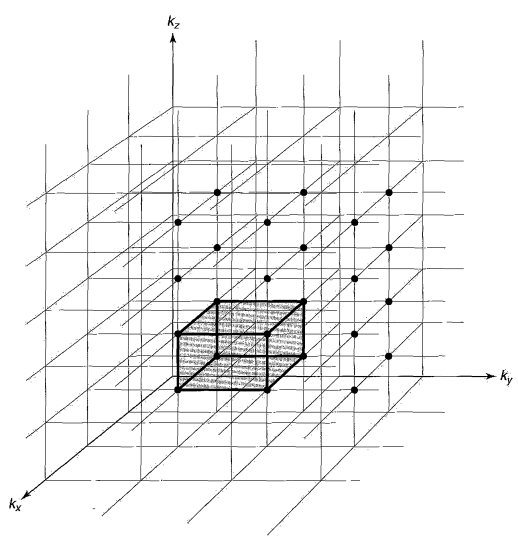
\includegraphics[width=0.75\linewidth]{grid.png}
\end{center}
Each intersection point represents a distinct one-particle stationary state.
Obviously, each block on this grid occupies a volume of ``$k$ space'' given
by
\[ \frac{\pi^3}{\ell_x\ell_y\ell_z} = \frac{\pi^3}{V} \]
where $V$ is the volume of the object itself.

Because electrons are fermions, and a maximum of 2 of them can occupy any
given state at a time, if left to settle, electrons will fill up an octant
of a sphere in $k$ space, whose radius ($k_F$, the \emph{Fermi momentum}) is
determined by the volume needed for each pair of electrons:
\begin{align*}
	\frac{1}{8} \left( \frac{4}{3} \pi k_F^3 \right)
	&= \frac{Nq}{2} \left( \frac{\pi^3}{V} \right)\\
	\implies k_F &= (4\rho\pi^2)^{1/3}\\
		     &: \rho \equiv \frac{Nq}{V}
\end{align*}
We call $\rho$ the free electron density, or the number of free electrons per
unit volume.\\
The boundary separating the occupied and unoccupied states (that is, the
boundary ad the edge of the sphere of filled states) is called the
\emph{Fermi surface}, and it has a corresponding energy called the
\emph{Fermi energy}. For a free electron gas,
\[ E_F = \frac{\hslash^2}{2m}(3\rho\pi^2)^{1/3} \]
To find the total energy, we can consider an infinite number of spherical
shells, of width $\d k$. The number of electron states in such a shell is
given by
\[ \frac{2[(1/2)\pi k^2\d k]}{\pi^3/V} = \frac{V}{\pi^2}k^2\d k \]
If each state carries the energy $\frac{\hslash^2 k^2}{2m}$, then the energy
of the shell is
\[ \d E = \frac{\hslash^2 V}{2\pi^2 m}k^4\d k \]
Thus, the total energy is found by integrating:
\begin{align*}
	E_{tot} &= \int_0^{k_F} k\d E\\
		&= \frac{\hslash^2 V}{2\pi^2 m} \int_0^{k_F} k^4 \d k\\
		&= \frac{\hslash^2 k_F^5 V}{10\pi^2 m}\\
		&= \frac{h^2(3\pi^2Nq)^{5/3}}{10\pi^2m}V^{-2/3}
\end{align*}
We can think of this quantum mechanical energy like the internal thermal energy
of an ordinay gas, especially in the sense that it exerts some pressure on the
walls: if the box expands by some amount (call it $\d V$), the total energy
decreases:
\begin{align*}
	\d E_{tot} &= -\frac{2}{3} \frac{\hslash^2(3\pi^2Nq)^{5/3}}{10\pi^2m}
			V^{-5/3}\d V\\
			&=  -\frac{2}{3} E_{tot}\frac{\d V}{V}
\end{align*}
This shows up as work done on the outside ($\d W = P \d V$), by some quantum
pressure $P$, where
\begin{align*}
	P &= \frac{2}{3} \frac{E_{tot}}{V}\\
	  &= \frac{2}{3} \frac{\hslash^2 k_F^5}{10\pi^2 m}\\
	  &= \frac{(3\pi^2)^{2/3}\hslash^2}{5m}\rho^{5/3}
\end{align*}
Thus, for every solid, ignoring both electron-electron interaction and
thermal motion, there must be some strictly quantum mechanical internal
stabilizing pressyre. This is usually called the \emph{degeneracy pressure}.

\subsubsection{Band Structure}
We can obviously improve on our last model/approximation in a lot of ways, but
for now we'll only look at one: we'll say that there are forces being exerted
on the electrons by regularly spaced, positive, stationary nuclei. The
actual shape isn't important (for us now), the important part is that it
is periodic, or that
\[ V(x+a) = V(x) \]
for some constant $a$.
\begin{thm}[Bloch's theorem]
	Solutions to the Schr\"odinger equation,
	\[ -\frac{\hslash^2}{2m}\der{^2\psi}{x^2} + V(x)\psi = E\psi \]
	for a periodic $V(x)$ can be taken to satisfy the condition
	\[ \psi(x+a) = e^{iKa}\psi(x) \]
	for some constant $K$ independent of $x$ (but potentially dependent on
	$E$).
\end{thm}
\begin{proof}
	Let $D$ be the displacement operator:
	\[ D f(x) = f(x+a) \]
	For a periodic potential, $D$ commutes with the Hamiltonian:
	\[ [D,H] = 0 \]
	Thius, $\exval{D}$ is time-independent and we can find simultaneous
	eigenstates of $D$ and $H$, so
	\[ D\psi = \psi(x+a) = \lambda\psi(x) \]
	Since $\lambda$ cannot be 0, like any nonzero complex number, it can
	be expressed as
	\[ \lambda = e^{iKa} \]
	for some constant $K$.
\end{proof}
Before we go back to our actual problem, we need to talk about $K$. Although
no real solid is infinite, meaning no real potential function is foreer
periodic, when we're talking about solids on the order of Avogadro's number
(or multiples or orders of magnitude thereof), the edge effects aren't going
to affect the behavior of the deep-inside electrons. We can do some
minor math trickery: If we wrap the x-axis in a circle and connect it to its
tail after a large number of periods ($N\sim10^{23}$), we can formally impose
the boundary condition:
\begin{align*}
	\psi(x+Na) &= \psi(x)\\
	e^{iNKa}\psi(x) &= \psi(x)\\
	e^{iNKa} &= 1\\
	NKa &= 2\pi n\\
	K &= \frac{2\pi n}{Na}
\end{align*}
Where $n$ can be any positive or negative integer (including 0). This means
that $K$ must also be a real number.

Back to our periodic potential: the simplest version of this we can envision
is a \emph{Dirac comb}, consisting of evenly-spaced Dirac delta functions:
\[ V(x) = \alpha \sum_{i=0}^{N-1} \delta(x-ia) \]
In the region $0<x<a$, $V(x)=0$, so the Schr\"odinger equation there goes to
\begin{align*}
	-\frac{\hslash^2}{2m}\der{^2\psi}{x^2} &= E\psi\\
	\der{^2\psi}{x^2} &= -k^2\psi\\
	&:k=\frac{\sqrt{2mE}}{\hslash}
\end{align*}
The general solution is relatively easy to find:
\[ \psi(x) = A\sin(kx) + B\cos(kx) \]
According to Bloch's theorem, the wave function in the cell just left of the
origin (at $x-a$, or $-a<x<0$) is
\[ \psi(x) = e^{-iKa}[A\sin(k(x+a)) + B\cos(k(x+a))] \]
If $\psi(x=0)$ is to be continuous, we must have
\[ B = e^{-iKa}[A\sin(ka)+B\cos(ka)] \]
But its derivative still suffers a discontinuity, which is proportional to the
strength of the delta function ($\alpha$):
\begin{align*}
	kA - e^{-iKa}k[A\cos(ka)-B\sin(ka)]&=\frac{2m\alpha}{\hslash^2}B\\
	A\sin(ka) &= [e^{iKa}-\cos(ka)]B
\end{align*}
Substituting this with the solution for $B$:
\begin{gather*}
	[e^{iKa}-\cos(ka)][1-e^{-iKa}\cos(ka)]+e^{-iKa}\sin^2(ka) =
	\frac{2m\alpha}{2\hslash^2 k}\sin(ka)\\
	\cos(Ka)=\cos(ka)+\frac{m\alpha}{\hslash^2 k}\sin(ka)
\end{gather*}
This is a super important result. It determines all possible values of $k$,
and thus the allowed energies. To make things a little simpler, we can
define two constants:
\begin{align*}
	z \equiv ka && \beta \equiv \frac{m\alpha a}{\hslash^2}
\end{align*}
So that we can write the RHS of that equation as
\[ f(z) = \cos(z)+\beta\frac{\sin(z)}{z} \]
If we were to graph $f(z)$, we would find that it sometimes strays outside of
the range $(-1,1)$, where there is no possibility of solving our important 
defining euqation---these gaps represent forbidden energies, separated by bands
of allowed energies. Energies are quantized, but at scales large enough to
care about, virtualy any energy level is allowed in the bands.

\section{Applications and Approximation Methods}

\subsection{Time-Independent Perturbation Theory}
\subsubsection{Nondegenerate Perturbation Theory}
Perturbation theory is a method of approximation which allows us to approximate
solutions to hard Hamiltonians by considering them as simpler Hamiltonians
which we know the solutions to (the \emph{unperturbed case}), with a small
change, or \emph{perturbation}. We do this by writing the difficult Hamiltonian
as a linear combination of 2 terms, the original (unperturbed) Hamiltonian,
$H_0$, and the perturbation, $H'$:
\[ H = H_0 + \lambda H' \]
We can then write $\psi_n$ and $E_n$ as a power series in $\lambda$:
\begin{align*}
	\psi_n &= \psi_n^{(0)} + \lambda\psi_n^{(1)} + \lambda^2\psi_n^{(2)}
		+ \cdots\\
	E_n &= E_n^{(0)} + \lambda E_n^{(1)} + \lambda^2E_n^{(2)}
		+ \cdots\\
\end{align*}
We call $E_n^{(1)}$ and $\psi_n^{(1)}$ the \emph{first-order corrections} to
the energy and wae function, respectively.\\
If we apply the Hamiltonian $H$ to this, we can find some cool stuff:
\begin{align*}
	(H_0+\lambda H')
	[\psi_n^{(0)} &+ \lambda\psi_n^{(1)} + \lambda^2\psi_n^{(2)} +
	\cdots]\\
	&= (E_n^{(0)} + \lambda E_n^{(1)} + \lambda^2E_n^{(2)} + \cdots)
	[\psi_n^{(0)} + \lambda\psi_n^{(1)} + \lambda^2\psi_n^{(2)} +
	\cdots]
\end{align*}
If we collect powers of $\lambda$, then we can write this as
\begin{align*}
	H_0\psi_n^{(0)} &+
	\lambda(H_0 \psi_n^{(1)} + H' \psi_n^{(0)}) +
	\lambda^2(H_0\psi_n^{(2)} + H' \psi_n^{(1)}) + \cdots\\
	&= E_n^{(0)}\psi_n^{(0)} +
	\lambda(E_n^{(0)}\psi_n^{(1)} + E_n^{(1)}\psi_n^{(0)}) +
	\lambda^2(E_n^{(0)}\psi_n^{(2)} + E_n^{(1)}\psi_n^{(1)}) + \cdots
\end{align*}
We can separate these then by order. The lowest order ($\lambda^0$) gives us
the unperturbed Schr\"odinger equation:
\[ H_0\psi_n^{(0)} = E_n^{(0)}\psi_n^{(0)} \]
The first order terms ($\lambda^1$) give us the Schr\"odinger equation for the
first-order correction:
\[ H_0\psi_n^{(1)} + H'\psi_n^{(0)} =
	E_n^{(0)}\psi_n^{(1)} + E_n^{(1)}\psi_n^{(0)} \]
The second-order terms ($\lambda^2$) give us the Schr\"odinger equation for the
second-ordder correction:
\[ H_0\psi_n^{(2)} + H'\psi_n^{(1)} =
E_n^{(0)}\psi_n^{(2)} + E_n^{(1)}\psi_n^{(1)} + E_n^{(2)}\psi_n^{(0)} \]

And that's as far as we'll go, we usually don't need anything past the
second-order correction term. Really, $\lambda$ was just to keep track of the
orders, but we can just say that $\lambda=1$ always and not have to worry about
it.

\paragraph{First-Order Corrections}
We can take the inner product of the first-order equation from above,
\[ H_0\psi_n^{(1)} + H'\psi_n^{(0)} =
	E_n^{(0)}\psi_n^{(1)} + E_n^{(1)}\psi_n^{(0)} \]
with the unperturbed wave function $\psi_n^{(0)}$:
\begin{align*}
	\braket{\psi_n^{(0)}}{H_0\psi_n^{(1)}} +
	\braket{\psi_n^{(0)}}{H'\psi_n^{(0)}} &=
		E_n^{(0)} \braket{\psi_n^{(0)}}{\psi_n^{(1)}} +
		E_n^{(1)} \cancelto{1}{\braket{\psi_n^{(0)}}{\psi_n^{(0)}}}\\
\end{align*}
Because $H_0$ is Hermitian, we can equate
\[ \braket{\psi_n^{(0}}{H_0\psi_n^{(1)}} =
	\braket{H_0\psi_n^{(0)}}{\psi_n^{(1)}} =
	\braket{E_n^{(0)}\psi_n^{(0)}}{\psi_n^{(1)}} =
	E_n^{(0)} \braket{\psi_n^{(0)}}{\psi_n^{(1)}}
\]
This will cancel out the first left term and the first right term.
Solving for $E_n^{(1)}$, then we find that
\[ E_n^{(1)} = \brak{\psi_n^{(0)}}H'\bket{\psi_n^{(0)}} \]
This is the \emph{first-order correction to the energy}.

But what happens to the wave function? We can re-write our first-order equation
as
\[ \left(H_0-E_n^{(0)}\right)\psi_n^{(1)} =
	-\left(H'-E_n^{(1)}\right)\psi_n^{(0)} \]
If we take the inner product with the unperterbed wave function with
the quantum number $\ell$, $\psi^{(0)}_\ell$:
\begin{align*}
	\brak{\psi_\ell^{(0)}}H_0-E_n^{(0)}\bket{\psi_n^{(1)}} &=
		E_n^{(1)}\braket{\psi_\ell^{(0)}}{\psi_n^{(0)}} -
		\brak{\psi_\ell^{(0)}}H'\bket{\psi_n^{(0)}}\\
	\left(E_\ell^{(0)}-E_n^{(0)}\right)
	\braket{\psi_\ell^{(0)}}{\psi_n^{(1)}} &=
		E_n^{(1)}\braket{\psi_\ell^{(0)}}{\psi_n^{(0)}} -
		\brak{\psi_\ell^{(0)}}H'\bket{\psi_n^{(0)}}\\
\end{align*}
If $n=\ell$, the LHS comes out to 0, and we'd just end back up with the first
order energy correction. So instead, we want to take $n\neq\ell$. Remember that
any wave function can be written as a linear combination of other wave
functions, such that
\[ \bket{\psi_n^{(1)}} = \sum_{n\neq m} c_{nm}\bket{\psi_m^{(0)}} \]
So we can write the first inner product on the left-hand side of the equation
above as
\begin{align*}
	\braket{\psi_\ell^{(0)}}{\psi_n^{(1)}} &=
		\sum_{n\neq m} c_{nm}\braket{\psi_\ell^{(0)}}{\psi_m^{(0)}}\\
		&= c_{n\ell}
\end{align*}
Substituting this back into the equation and solving for $c_{n\ell}$,
\begin{align*}
	\left(E_\ell^{(0)}-E_n^{(0)}\right)c_{n\ell} &=
	-\brak{\psi_\ell^{(0)}}H'\bket{\psi_n^{(0)}}\\
	c_{n\ell} &= \frac{\brak{\psi_\ell^{(0)}}H'\bket{\psi_n^{(0)}}}
		{E_n^{(0)}-E_\ell^{(0)}}
\end{align*}
Taking $\ell\to m$, this means that
\[
	\psi_n^{(1)} = \sum_{m\neq n}
		\frac{\brak{\psi_m^{(0)}}H'\bket{\psi_n^{(0)}}}
		{E_n^{(0)}-E_m^{(0)}}\psi_m^{(0)}
\]
This is the \emph{first-order correction to the wave function}. This is safe
as long as the unperturbed energy spectrum is nondegenerate---if it is
degenerate, we need to look at degenerate perturbation theory, but that'll
come in the next section. Note: in perturbation theory, the energies are
usually pretty accurate, but the wave functions are notoriously not great.

\paragraph{Second-Order Corrections}
We can do basically the same thing for the second-order correction terms, but
instead taking the inner product with with $\brak{\psi_n^{(0)}}$ and the
second-order equation:
\begin{align*}
	\cancelto{0}{
	\brak{\psi_n^{(0)}} H_0 \bket{\psi_n^{(2)}}} +
	\brak{\psi_n^{(0)}} H'  \bket{\psi_n^{(1)}}  &=\\
	\cancelto{0}{
	E_n^{(0)} \braket{\psi_n^{(0)}}{\psi_n^{(2)}}} &+
	\cancelto{0}{
	E_n^{(1)} \braket{\psi_n^{(0)}}{\psi_n^{(1)}}}  +
	E_n^{(2)} \braket{\psi_n^{(0)}}{\psi_n^{(0)}}
\end{align*}
We can once again exploit that any state can be written as a sum of other
states, like we did before:
\begin{align*}
	E_n^{(2)} &= \brak{\psi_n^{(0)}} H' \bket{\psi_n^{(1)}}\\
		  &= \sum_{m\neq n} c_{mn}
		     \brak{\psi_m^{(0)}} H' \bket{\psi_n^{(0)}}\\
		  &= \sum_{m\neq n} \frac{
		     \brak{\psi_m^{(0)}} H' \bket{\psi_n^{(0)}}
		     \brak{\psi_m^{(0)}} H' \bket{\psi_n^{(0)}}}
		     {E_n^{(0)} - E_m^{(0)}}\\
	E_n^{(2)} &= \sum_{m\neq n}\frac{
		\abs{\brak{\psi_m^{(0)}} H' \bket{\psi_n^{(0)}}}^2}
		{E_n^{(0)}-E_m^{(0)}}
\end{align*}

\begin{eg}
	Consider a one-dimensional infinite square well. Find the first and
	second order corrections to energy and the first-order correction to
	the wave function if there is a perturbation with the Hamiltonian:
	\begin{enumerate}
		\item $H' = V_0$
		\item $H' = \begin{cases}V_0,&0<x<a/2\\0,&a/2<x<a\end{cases}$
	\end{enumerate}
	\textbf{Solution.}
	\begin{enumerate}
	\item
		We already know the unperturbed wave function and
		energy:
		\begin{align*}
			\psi_n^{(0)} &= \sqrt{\frac{2}{a}}
				\sin\left(\frac{n\pi}{a} x\right)\\
			E_n^{(0)} &= \frac{\hslash^2 \pi^2 n^2}{2 m a^2}
		\end{align*}
		The first-order energy term is pretty easy to figure out:
		\begin{align*}
			E_n^{(1)}&=\brak{\psi_n^{(0)}} H' \bket{\psi_n^{(0)}}\\
				 &=V_0 \braket{\psi_n^{(0)}}{\psi_n^{(0)}}\\
				 &= V_0
		\end{align*}
		By extension, the first-order wave function correction is
		relatively easy to find:
		\begin{align*}
			\psi_n^{(1)} &= \sum_{n\neq m} \frac{
				\brak{\psi_m^{(0)}} H' \bket{\psi_n^{(0)}}}{
				E_n^{(0)}-E_m^{(0)}}\bket{\psi_m^{(0)}}\\
			&= V_0\sum_{n\neq m} \frac{
				\braket{\psi_m^{(0)}}{\psi_n^{(0)}}}{
				E_n^{(0)}-E_m^{(0)}}\bket{\psi_m^{(0)}}\\
			&= 0
		\end{align*}
		Again, by extension,
		\begin{align*}
			E_n^{(2)} &= \sum_{m\neq n}\frac{
			\abs{\brak{\psi_m^{(0)}} H' \bket{\psi_n^{(0)}}}^2}
			{E_n^{(0)}-E_m^{(0)}}\\
			&= 0
		\end{align*}
		Thus, we can write the energy and wave function as the sum of
		the first- and second-order corrections (which turns out to
		actually be the exact wave function, but don't always count
		on that):
		\begin{align*}
			E_n &= E_n^{(0)} + E_n^{(1)} + E_n^{(2)}\\
			    &= \frac{\hslash^2 \pi^2 n^2}{2 m a^2} + V_0\\
			\psi_n(x) &= \psi_n^{(0)}(x) + \psi_n^{(1)}(x)\\
				  &= \sqrt{\frac{2}{a}}
					\sin\left(\frac{n\pi}{a}x\right)
		\end{align*}
	\item
		We start in much the same way, but we can't quite make the
		same simplifcations as before:
		\begin{align*}
			E_n^{(1)}&=\brak{\psi_n^{(0)}} H' \bket{\psi_n^{(0)}}\\
				 &= \frac{2V_0}{a}\int_0^{a/2}\sin^2\left(
					\frac{n\pi x}{a}\right) \d x\\
					&= \frac{V_0}{2}
		\end{align*}
	\end{enumerate}
\end{eg}


\subsubsection{Degenerate Perturbation Theory}
Perturbation theory as we've written it doesn't always work out so well. If
the unperturned states are degenerate (ie. if there are 2+ distinct states that
share the same energy), then we can see clearly that the first-order correction
to the wave function and the second-order correction to energy blow up, but
we're going to start from the beginning, because it's possible we can't even
trust our first-order energy correction.\\
Suppose we have $N$ states, all with the same energy $E_n$. Recall that any
wave function can be written as a linear combination of these degenerate
states:
\[ \psi_n^{(0)} = \sum_{a=1}^N c_{n,a}\psi_{n,a}^{(0)} \]
We can write this as a vector with the basis of these eigenstates:
\[
	\psi_n^{(0)} =
	\begin{pmatrix}
		c_{n,1}\\
		c_{n,1}\\
		\vdots\\
		c_{n,N}
	\end{pmatrix}
\]
If we do so, we can write the operators ($H_0$ and $H'$) as matrices.
In general, the perturbation will ``lift'' the degeneracy. This means that
when we lift $\lambda$ from $0\to1$, the shared unperturbed energy will split
into some number of distinct energies (usually $N$). When we turn off the
perturbation, the states return to that number of orthogonal linear
combinations, but we can't know ahead of time what these ``good'' linear
combinations will be, so we can't calculate the first-order energy in the
same way, because we won't know what linear combination of unperturbed states
to use. For now, we'll write the linear combinations in terms of generic
scalar values. Using the first-order equation from earlier,
\[
	H_0\psi_n^{(1)} + H'\psi_n^{(0)} =
		E_n^{(0)}\psi_n^{(1)} + E_n^{(1)}\psi_n^{(0)}
\]
and again taking the inner product with $\brak{\psi_{n,a}^{(0)}}$, we get
\begin{align*}
	\cancelto{0}{
	\brak{\psi_{n,a}^{(0)}}H_0\bket{\psi_{n}^{(1)}}} +
	\brak{\psi_{n,a}^{(0)}}H' \bket{\psi_{n}^{(0)}} &=
	\cancelto{0}{
	E_n^{(0)}\braket{\psi_{n,a}^{(0)}}{\psi_{n}^{(1)}}} +
	E_n^{(1)}\braket{\psi_{n,a}^{(0)}}{\psi_{n}^{(0)}}\\
	\brak{\psi_{n,a}^{(0)}}H'\bket{\psi_{n}^{(0)}} &=
	E_n^{(1)}\braket{\psi_{n,a}^{(0)}}{\psi_n^{(0)}}\\
\end{align*}
Using the orthonormality condition, and the rule we established earlier about
linear combinations, we can write this as
\begin{align*}
	c_1\brak{\psi_{n,a}^{(0)}}H'\bket{\psi_{n,a}^{(0)}} +
	c_2\brak{\psi_{n,a}^{(0)}}H'\bket{\psi_{n,b}^{(0)}} &=
	c_1 E_n^{(1)}\\
	c_1W_{aa} + c_2W_{ab} &= c_1E^{(1)}
\end{align*}
$W_{ij}$ are matrix elements for some matrix $W$.
We can pick solutions to an earlier form of that equation,
\[ \brak{\psi_n^{(0)}}H'\bket{\psi_n^{(0)}} = 
	\brak{\psi_n^{(0)}}E_n^{(1)}\bket{\psi_n^{(0)}} 
\]
Such that the matrix $W$ is diagonalized. To do so:
\[ \brak{\psi_n^{(0)}}(H'-IE_n^{(1)})\bket{\psi_n^{(0)}} = 0 \]
This is just a standard eigenvalue equation. For a given set of $n$s (I think?)
then for 2-fold degeneracy,
\[
	\begin{pmatrix}
		W_{11} - E_n^{(1)} & W_{12}\\
		W_{21} & W_{22} - E_n^{(1)}
	\end{pmatrix}
	\begin{pmatrix}
		c_1 \psi_{n,1}\\
		c_2 \psi_{n,2}
	\end{pmatrix}
	= 0
\]
[I don't know if I understand the explanations here]

\begin{eg}
	Consider a 3-dimensional square well (ie. a particle in a box).
	Assume the perturbation Hamiltonian is given by
	\[ H' = \begin{cases}
			V_0, & 0<x<a/2, 0<y<a/2, 0,z,a/2\\
			0,   & \text{Otherwise}
		\end{cases}
	\]
	Find the first-order corrections to energy and wave function for the
	first excited state.\\
	\textbf{Solution.}
	The unperturbed wave function and energy, respectively, are given by:
	\begin{align*}
		\psi_{n_x,n_y,n_z}^{(0)} &= \left(\frac{2}{a}\right)^{3/2}
			\sin\left(\frac{n_x\pi}{a}x\right)
			\sin\left(\frac{n_y\pi}{a}y\right)
			\sin\left(\frac{n_z\pi}{a}z\right)\\
		E_{n_x,n_y,n_z}^{(0)} &= \frac{\hslash^2\pi^2}{a^2}\left(
			n_x^2+n_y^2+n_z^2\right)
	\end{align*}
	There is a clear problem: there are 3 possible first excited states:
	\begin{gather}
		n_x = 1, n_y = 1, n_z = 2\\
		n_x = 1, n_y = 2, n_z = 1\\
		n_x = 2, n_y = 1, n_z = 1
	\end{gather}
	By the problem statement, we can't know which one we're referring to.
	So we can set up a 3x3 $W$ eigenvalue matrix. I won't show the
	calculations for every term, but I will show one here and then show
	the full results:
	\begin{align*}
		W_{23}&=\brak{\psi_{1,2,1}^{(0)}}H'\bket{\psi_{2,1,1}^{(0)}}\\
		      &=\left(\frac{2}{a}\right)^3V_0\times\\
		      &\hspace{1.5em}\left[
			\int_0^{a/2}
				\sin\left(\frac{\pi x}{a}\right)
				\sin\left(\frac{2\pi x}{a}\right)\d x
			\int_0^{a/2}
				\sin\left(\frac{2\pi y}{a}\right)
				\sin\left(\frac{\pi y}{a}\right)\d y
			\int_0^{a/2}
				\sin^2\left(\frac{\pi z}{a}\right)\d z
		\right]\\
		&= \frac{16V_0}{9\pi^2}\\
		&= \frac{V_0}{4}K\\
		&: K = \frac{16}{9\pi^2}
	\end{align*}
	The full matrix is thus
	\[
		W = 
	\begin{pmatrix}
		1 & 0 & 0\\
		0 & 1 & K\\
		0 & K & 1
	\end{pmatrix}
	\frac{V_0}{4}
	\]
	The ``good'' states (ie. eigenvector solutions to the eigenvalue
	equations, I think) are then
	\begin{align*}
		\psi_1^{(0)} &= 
			\begin{pmatrix}1\\0\\0\end{pmatrix}&
			E_1^{(0)} &= \frac{V_0}{4}\\
		\psi_2^{(0)} &=
			\frac{1}{\sqrt{2}}\begin{pmatrix}0\\1\\1\end{pmatrix}&
			E_1^{(0)} &= \frac{V_0}{4}(1+K)\\
		\psi_3^{(0)} &=
			\frac{1}{\sqrt{2}}\begin{pmatrix}0\\1\\-1\end{pmatrix}&
			E_1^{(0)} &= \frac{V_0}{4}(1-K)\\
	\end{align*}
	It then makes sense for us to be able to calculate the first-order
	correction to the wave function. Which I won't do here.
\end{eg}


\subsection{The Variational Principle}
\subsubsection{Theory}
Perturbation theory is really great if we have a Hamiltonian really similar to
to the one we already know (ie. if the difference or perturbation is small).
In the case that we have Hamiltonians that are totally unfamiliar to us,
we can use other methods, like the \emph{Variational method}. This will
give us an upper bound for the ground state energy (and, possibly,
higher excited energies). This doesn't give us any information about the wave
function, though.
\begin{prop}
	For any square-integrable (ie. normalized) wave function,
	\[ E_{gs} \leq \brak{\psi}H\bket{\psi} = \exval{H} \]
\begin{proof}
	The eigenfunctions of $H$ form a complete orthonormal basis, so we
	can write any $\psi$ in terms of them:
	\[ \bket{\psi} = \sum_n c_n\bket{\psi_n} \]
	for
	\[ H\psi_n = E_n\psi_n \]
	Since $\psi$ is normalized,
	\begin{align*}
		1 &= \braket{\psi}{\psi}\\
		  &= \sum_{n,m}c_m^\star c_n
			\cancelto{\delta_{m,n}}{\braket{\psi_m}{\psi_n}}\\
		&= \sum_n \abs{c_n}^2
	\end{align*}
	Thus,
	\begin{align*}
		\exval{H} =
		\brak{\psi}H\bket{\psi} &= \sum_{n,m} c_m^\star c_n
		\cancelto{E_n\delta_{m,n}}{\brak{\psi_m}H\bket{\psi_n}}\\
		&= \sum_n E_n\abs{c_n}^2
	\end{align*}
	The ground state energy is the smallest eigenvalue, meaning, by
	definition, $E_{gs} \leq E_n$. So for any other $n$,
	\[
		\exval{H} \geq E_{gs}\sum_n\abs{c_n}^2 = E_{gs}
	\]
\end{proof}
\end{prop}
If we want to find an upper bound to the ground state energy, then, we can
pick any normalized wave function. If we want to get a more accurate upper
bound, we can minimize the wave function in terms of one or moreof its
parameters. For example, for a Gaussian wave function,
\[ \psi(x) = Ae^{-bx^2} \]
We can minimize the energy in terms of the parameter $b$:
\[ \pd{b}\exval{H(b)} = 0 \]
will give the $b = b_0$ where the energy of this wave function is at a minimum.
\\~\\
How do we choose a trial wave function? We want one that approaches 0 as
$x \to \infty$, and it should be at a maximum when $V(x)$ is at a minimum.
Ideally, it should have no nodes.
\\~\\
We can use a trick when we need to calculate the kinetic energy portion of
the Hamiltonian:
\begin{align*}
	\brak{\psi}\pd[2]{x}\bket{\psi} &= \braket{\psi}{\pder{^2\psi}{x^2}}\\
	&= \int_{-\infty}^{\infty} \psi^\star\psi''\d x
	& u = \psi^\star,\d v=\psi''\d x\\
	&& \d u = (\psi^\star)', v = \psi'\\
	&= \psi^\star\psi''\bigg|_{-\infty}^\infty -
	\int_{-\infty}^{\infty} \psi(\psi^\star)'\d x\\
	&= -\int_{-\infty}^\infty \abs{\psi(x)}^2\d x
\end{align*}
So when we're looking at the kinetic energy term of a Hamiltonian, we can find
it more simply with
\[
\exval{T} = \frac{\hslash^2}{2m}\int_{-\infty}^\infty\abs{\der{\psi}{x}}^2\d x
\]
\\~\\
If we want to find an approximation for the first excited state using the
variational method:
\begin{enumerate}
	\item Find a good $\psi_g(x)$ to approximate the ground state
		wave function
	\item Find a trial wave function that's orthogonal to $\psi_g(x)$
	\item Minimize $\psi(x)$ with respect to one or more of its parameters
	\item Find the expectation value of the Hamiltonian
\end{enumerate}
The value that we find from this is an approximation, but doesn't provide any
bounds (we can't tell if it's an over-approximation or an under-approximation).
The exception is for Hamiltonians with a symmetric $V$ (ie. $V(x) = V(-x)$).
For a symmetric $V$, all states must be either even or odd
(ie. $\psi(-x) = \psi(x)$ or $\psi(-x) = -\psi(x)$, respectively), where
$\braket{\text{even}}{\text{odd}} = 0$. The ground state is always even, so the
first excited state must be odd.
\\~\\
\paragraph{Perturbation Theory and the Variational Method}
Consider a Hamiltonian like the one we're used to seeing with Perturbation
theory, $H = H_0 + H'$. We can use the ground-state eigenstate of $H_0$,
$\bket{\psi_g^{(0)}}$, as the trial wafe functions for the variational
calculations:
\begin{align*}
	E_g &\leq \brak{\psi_g^{(0)}}H\bket{\psi_g^{(0)}}\\
	    &\leq \brak{\psi_g^{(0)}}H_0\bket{\psi_g^{(0)}} +
		  \brak{\psi_g^{(0)}}H\bket{\psi_g^{(0)}}\\
	E_g &\leq E_g^{(0)} + E_g^{(1)}
\end{align*}
This proves a claim we made earlier: the first-order equation in perturbation
theory is \emph{always} an over-estimate (which means the second-order
correction is always negative and will always bring it back down).

\subsubsection{Examples}

\begin{eg}
	Find the upper limit to the ground state energy for the 1-dimensional
	harmonic oscillator.\\
	\textbf{Solution.}
	Recall that the
	potential function for a harmonic oscillator is roughly parabolic,
	with a Hamiltonian of
	\[ H = -\frac{\hbar^2}{2m}\pder{^2}{x^2} + \frac{m}{2}\omega^2 x^2 \]
	We can choose a simple Gaussian function as our trial wave function:
	\[ \psi(x) = Ae^{-bx^2} \]
	Applying the Hamiltonian operator,
	\[ H\bket{\psi} = -\frac{\hbar^2}{2m}2bAe^{-bx^2}(2bx^2-1) +
		\frac{m}{2}\omega^2 x^2 Ae^{-bx^2} \]
	We can find the normalization constant $A$:
	\begin{align*}
		1 &= \braket{\psi}{\psi}\\
		  &= \int_{-\infty}^\infty \abs{A}^2e^{-bx^2}\d x\\
		  &= \abs{A}^2\sqrt{\frac{\pi}{2b}}\\
		A &= \left(\frac{2}{\pi b}\right)^{1/4}
	\end{align*}
	Similarly, we can find the expectation value of $H$ and minimize it
	in terms of $b$:
	\begin{align*}
		\exval{H} &= \brak{\psi}H\bket{\psi}\\
			  &=\frac{\hslash^2}{2m}b+\frac{m\omega^2}{8b}
		\\~\\
		\pder{\exval{H}}{b} &=
		\frac{\hslash^2}{2m} - \frac{m\omega^2}{8b^2} = 0\\
		\implies b_0 &= \frac{m\omega}{2\hslash}
	\end{align*}
	If we plug this minimum $b_0$ into the Hamiltonian expectation value,
	we can find our upper bound for the ground-state energy:
	\begin{align*}
		\exval{H(b_0)} &=
			\frac{\hslash^2}{2m}b_0 + \frac{m\omega^2}{8b_0}\\
			&= \frac{\hslash\omega}{4} + \frac{\hslash\omega}{4}\\
			&= \frac{\hslash\omega}{2} \geq E_g
	\end{align*}
	We actually know the ground-state energy in this case, and it
	actually turns out that the equality in this case is true, because
	we picked the exact correct wave function, but that won't always be the
	case.
\end{eg}

\begin{eg}
	Find the upper limit to the ground state energy for the 1-dimensional
	infinite well using a triangular wave function.\\
	\textbf{Solution.}
	A triangular wave function will look like
	\[
		\begin{cases}
			Ax, & 0\leq x \leq a/2\\
			A(a-x), & a/2 < x <\leq a
		\end{cases}
	\]
	There are no parameters to minimize with respect to here. First,
	we can find the normalization constant $A$:
	\begin{align*}
		1 &= \braket{\psi}{\psi}\\
		  &= \abs{A}^2\int_0^{a/2}x^2\d x +
		     \abs{A}^2\int_{a/2}^a(a-x)^2\d x\\
		  &= A^2\frac{a^3}{12}\\
		A &= \sqrt{\frac{12}{a^3}}\\
		  &= \frac{2}{a}\sqrt{\frac{3}{a}}
	\end{align*}
	Next, we can find the expectation value of $H$, and plug in the
	normalization constant we found. Since there's nothing to minimize
	with respect to, our result here will be the upper limit.
	\begin{align*}
		\exval{H} &= \brak{\psi}H\bket{\psi}\\
			  &= -\frac{\hslash^2}{2m}
				\brak{\psi}\pd[2]{x}\bket{\psi}\\
			&= -\frac{\hslash}{2m}
				\int_0^a \abs{\der{\psi}{x}}^2\d x\\
			&= \frac{\hslash^2 A^2 a}{2m}\\
			&= \frac{12\hslash^2}{2ma^2} \geq E_g
	\end{align*}
	We know the actual value of the ground state energy:
	\[ E_g = \frac{\hslash^2\pi^2}{2ma^2} \]
	12 is greater than $\pi^2$, so our estimate of an upper limit is
	accurately an overestimate.
\end{eg}

\subsection{A Finer Look at Hydrogen}
\subsubsection{The Fine Structure of Hydrogen}
	We've already solved a basic model for the hydrogen atom. But it turns
	out that's not the full story: the energy levels of the hydrogen atom
	split finely even for individual states. We can explain that with
	two things: a relativistic correction, and spin-orbit coupling. Because
	this is such a small difference from the standard Bohr energies
	(on the order of $\alpha = \frac{1}{137}$, we can use perturbation
	theory to examine this fine structure splitting. Note that when I write
	things in terms of $\alpha$, I'm writing from my lecture notes and I'm
	not sure exactly how accurate it is. Everything else is from the
	textbook.
\paragraph{The Relativistic Correction}
	The kinetic energy
	term in the Hamiltonian is given by
	\[ T = \frac{p^2}{2m} = -\frac{\hslash^2}{2m}\del^2 \]
	But we know that in relativity, th expression for kinetic energy is a
	little different. We know that the relativistic energy of a particle is
	\[ E^2 = (cp)^2 + (mc^2)^2\]
	And we know that the relativistic kinetic energy of a particle is
	\[ T = E - mc^2 \]
	Combining these, we can find at least an approximation of the
	relativistic kinetic energy in terms of momentum:
	\begin{align*}
		T &= E - mc^2\\
		  &= \sqrt{(cp)^2-(mc^2)^2} - mc^2\\
		  &= mc^2\sqrt{1+\frac{p^2}{m^2}} - mc^2\\
		  &\approx mc^2\left(1+\frac{p^2}{2m^2c^2} -
			\frac{1}{8}\left(\frac{p}{mc}\right)^4 +
			\mathcal{O}(p^6)\right)\\
		T &\approx \frac{p^2}{2m} - \frac{p^4}{8m^3c^2} + \cdots
	\end{align*}
	For $p\ll m$, this is sufficient. We can see that this is simply the
	non-relativistic kinetic energy plus some first-order correction. In
	terms we're used to in perturbation theory,
	\[ H_{rel}' = -\frac{p^4}{8m^3c^2} \]
	The correction to $E_n$ is the expectation value of $H'$ in the
	unperturbed state. Note that since $p$ is Hermitian,
	$(p^2)^\dagger = p^2 \implies p^4 = (p^2)^\dagger p^2$.
	\begin{align*}
		E_{rel}^{(1)} &= -\frac{1}{8m^3c^2}\brak{\psi}p^4\bket{\psi}\\
			      &= -\frac{1}{8m^4c^2}
				\brak{\psi}(p^2)^\dagger p^2\bket{\psi}\\
			      &= -\frac{1}{8m^3c^2}\braket{p^2\psi}{p^2\psi}
	\end{align*}
	We can extrapolate from the Schr\"odinger equation to say that
	\[ p^2\bket{\psi} = 2m(E_n^{(0)} - V)\bket{\psi} \]
	We know that in the unperturbed Hamiltonian for the hydrogen atom,
	\[ V(r) = -\frac{e^2}{4\pi\epsilon_0 r} = -\frac{\alpha\hslash c}{r} \]
	So, for our first-order correction,
	\begin{align*}
		E_r^{(1)} &= -\frac{1}{2mc^2}\exval{(E_n^{(0)}-V)^2}\\
			  &= -\frac{1}{2mc^2}
		\left[(E_n^{(0)})^2-2E_n^{(0)}\exval{V}+\exval{V^2}\right]\\
			&= -\frac{1}{2mc^2}\left[
		(E_n^{(0)})^2 + 2E_n^{(0)}\alpha\hslash c\exval{\frac{1}{r}} +
		(z\hslash c)^2\exval{\frac{1}{r^2}}\right]
	\end{align*}
	We know from before that
	\[ \exval{\frac{1}{r}} = \frac{1}{n^2 a_0} \]
	Where $a_0$ is the Bohr radius,
	\[ a_0 = \frac{\hslash}{\alpha mc} \]
	There's a problem in Griffiths about calculating the other expectation
	value, but I'll just show the result here:
	\[ \exval{\frac{1}{r^2}} = \frac{1}{(\ell+1/2)n^3a_0^2} \]
	So, we can write the first-order relativistic corrections in full as
	\begin{align*}
		E_r^{(1)} &=
	-\frac{mc^2\alpha^4}{8n^4}\left[\frac{4n}{\ell+1/2} - 3\right]\\
	&= -\frac{(E_n^{(0)})^2}{2mc^2}\left[\frac{4n}{\ell+1/2}-3\right]
	\end{align*}
\paragraph{Spin-Orbit Coupling}
If we look at the motion of the particles from the perspective of the electron,
the proton is circling around it, setting up a magnetic field, $B$, in the
electron's reference frame, which exerts a torque on the electron. This
torque will try to align the electron's magnetic moment, $\vec{\mu}$, with the
magnetic field. The Hamiltonian for this is
\[ H' = \vec{\mu}\cdot\vec{B} \]
Recall that the magnetic dipole moment of spin for an electron is
\[ \vec{\mu} = -g_s\frac{e}{2m}\vec{S} \]
The magnetic lop of the effectively continuous loop formed by the proton can
be found using the Biot-Savart law:
\[ \vec{B} = \frac{\mu_0 I}{2r}\vhat{r} \]
With an effective current of
\[ I = \frac{e}{T} \]
where $T$ is the period of the orbit. The orbital angular momentum of the
electron in the fram of the nucleus is
\[ \vec{L} = rmv\vhat{r} = \frac{2\pi mr^2}{T}\vhat{r} \]
We can relate this with $\vec{B}$ using the identity
$c = 1/\sqrt{\mu_0\epsilon_0}$:
\[ \vec{B} = \frac{1}{4\pi\epsilon_0}\frac{e}{mc^2r^3}\vec{L} \]
This is an approximation---the proton is accelerating with respect to the
electron, meaning this boost isn't technically accurate. If we do it the
right way, we get basically the same answer, multiplied by a factor of
$1/2$:
\begin{align*}
	H'_{so} &= -\frac{1}{2}\vec{mu}\cdot\vec{B}\\
		&= \frac{e^2}{8\pi\epsilon_0}\frac{1}{m^2c^2r^3}
			\vec{S}\cdot\vec{L}
\end{align*}
This is the spin-orbit interaction. In the presence of spin-orbit coupling, the
Hamiltonian doesn't commute with $\vec{L}$ or $\vec{S}$ anymore, so the
spin and orbital angular momenta aren't conserved on their own, but it does
commute with $L^2$ and $S^2$, and the total angular momentum
($\vec{J} = \vec{L} + \vec{S}$) is conserved. In better words, the eigenstates
of $L_z$ and $S_z$ aren't very good eigenstates for our perturbation theory,
but eigenstates of $L^2$, $S^2$, $J^2$, and $J_z$ are.\\
The first-order energy correction can be given by
\begin{align*}
	E_{so}^{(1)} &= \frac{e^2}{8\pi\epsilon_0}\frac{1}{m^3c^2}
		\expval{\psi}{\frac{\vec{S}\cdot\vec{L}}{r^3}}{\psi}\\
		&= \frac{\alpha\hslash}{2m^2c}
			\exval{\frac{\vec{S}\cdot\vec{L}}{r^3}}\\
		&= \frac{\alpha\hslash}{2m^2c}
			\exval{\vec{S}\cdot\vec{L}}
			\exval{\frac{1}{r^3}}
\end{align*}
Remember that
\[ J^2 = (\vec{S}+\vec{L})^2 = S^2 + 2\vec{S}\cdot\vec{L} + L^2 \]
So,
\begin{align*}
	\vec{S}\cdot\vec{L} &= \frac{J^2-L^2-S^2}{2}\\
	&= \frac{\hslash^2}{2}\left[j(j+1) - \ell(\ell+1) - \frac{3}{4}\right]
\end{align*}
Note, the last term is technically $s(s+1)$, but for electrons, $s=1/2$.\\
Again, this is a problem in Griffiths, but we can also find the expectation
value for the other part:
\[ \exval{\frac{1}{r^3}} = \frac{1}{\ell(\ell+1/2)(\ell+1)n^3a_0^3} \]
Combining all of these:
\begin{align*}
	E_{so}^{(1)} &= \frac{\alpha\hslash^3}{2m^2c}
	\frac{j(j+1)-\ell(\ell+1)-3/4}{\ell(\ell+1/2)(\ell+1)n^3a_0^3}\\
	&= \frac{\left(E_n^{(0)}\right)^2}{mc^2}
	\left\{\frac{n[j(j+1)-\ell(\ell+1)-3/2]}
	{\ell(\ell+1)(\ell+1)n^3a_0^3}\right\}
\end{align*}
\paragraph{The Fine Structure}
The total corrections are on the order of $mc^2\alpha^4$. The full first-order
correction for the fine structure of hydrogen is thus
\begin{align*}
	E_{fs}^{(1)} &= \frac{mc^2}{8}\frac{\alpha^4}{n^4}\left(
	3-\frac{8n}{2j+1}\right)\\
	&= \frac{\left(E_n^{(0)}\right)^2}{2mc^2}\left(
	3-\frac{4n}{j+1/2}\right)
\end{align*}
For a given $\ell$, we know that $j$ can take values $\ell \pm 1/2$.
Combining this with the Bohr formula, we can find the full approximation for
the hydrogen atom including the first-order correction:
\begin{align*}
	E_{nj} &= E_n^{(0)} + E_{fs}^{(1)}\\
	       &= E_1^{(0)}\left[1+\frac{\alpha^2}{n^2}\left(\frac{n}{j+1/2}-
		\frac{3}{4}\right)\right]\\
		&= -\frac{13.6\mathrm{eV}}{n^2}
		\left[1+\frac{\alpha^2}{n^2}\left(\frac{n}{j+1/2}-
		\frac{3}{4}\right)\right]\\
\end{align*}
For a given $n$, states split according to their total angular momentum. The
fine structure breaks the degeneracy in $\ell$, but it preserves the degeneracy
in $j$. The quantum numbers we want to use to label the states are
are $n$, $\ell$, $s$, $j$, and $m_j$.

\subsubsection{Hyperfine Splitting}
The proton has spin, too.

\subsection{Splitting from Electric and Magnetic Fields}
\subsubsection{Electric Fields: The Stark Effect}
\subsubsection{Magnetic Fields: The Zeeman Effect}

\end{document}
